As a preface to the following numerical validation, it should be mentioned that each of the test cases consist of two-dimensional rectangular domains with no objects in these domains. To be blunt this is a worst case for LABFM, which is a meshless method designed for its effectiveness in `interesting' geometries.

\emph{And rectangles are not interesting.}

Having said that, although the computational time may be larger than if, say, a simple centred finite difference method had been used due to the much larger stencil sizes, the use of LABFM here still provides discretisations with the high accuracy we require for the validation of the ADCBCs discussed in the previous chapter. Beyond this, there is something to be said for applying these new boundary conditions under less well-trodden conditions: if it works under LABFM, one would expect it also to work under more traditional methods.





\section{Acoustic Bump}

\begin{figure}[t]
\centering
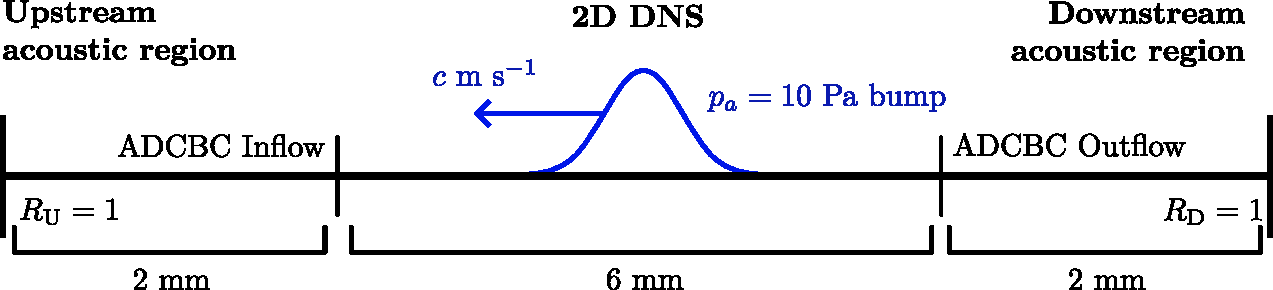
\includegraphics[scale=0.65]{assets/imgs/adcbc_bump_test.pdf}
\caption{The geometry and initialisation for the acoustic bump test case. Not drawn to scale.}
\label{fig:ac-bump-test}
\end{figure}

As our first test case, we model a Gaussian acoustic bump in a two-dimensional tube with two closed ends. The test case is initialised as a small bump in $J_1 \approx p' - ρ c u'$ (where the approximation comes from acoustic linearisation):
\begin{equation}
p_a(t = 0, x) = A \exp\left( - x^2 / d^2 \right)
\quad \text{and} \quad
u_a(t = 0, x) = p_a(t = 0, x) / ρ c
\end{equation}
such that the maximum pressure disturbance is $A = 10$ Pa and diameter $d = 2$ mm. This simple linear approximation also results in a small $J_5$ bump which we ignore. Alternate methods approximating this initial disturbance could also be used, although the provide little relevant improvement. Fluid properties are $u_{\rm{IN}} = 0.2$ m s$^{-1}$, $T_{\rm{IN}} = 298$ K and $p_{\rm{IN}} = 0.1$ MPa comprised of a single species with properties $W = 28$ kg kmol$^{-1}$, $Pr = 0.7$ and $c_p = 1100$ J kg$^{-1}$ K$^{-1}$. The resulting sound speed is $c \approx 348$ m s$^{-1}$. A 6 mm long central DNS region is used as well as up- and downstream acoustic regions modelled using ADCBCs on the inflow and outflow respectively, each modelling 2 mm of truncated tube. These essentially model two one-dimensional acoustic regions to the left and right of the flame. A diagram for this test case is shown in \fig{fig:ac-bump-test}. A sample rate of $δt_{\rm{sample}} \approx 0.25$ {\textmu}s is used for both ADCBCs and we use \nth{0} order interpolation (constant sample values) at the moment, for reasons discussed later. The horizontal top and bottom boundaries used in the DNS region are symmetric mirror boundaries, 1 mm apart. The LABFM discretisation uses $k = 4$ on gradients and Laplacians and $k_{\rm{HV}} = 6$ for $-Δ^2$ hyperviscosity filtering. In total, there are 1224 LABFM discretisation points in this domain processed by a single processor and 11 boundary nodes per boundary. With the linear acoustics equations in the acoustic regions being non-dispersive, we expect the Gaussian to retain its shape after each up- and downstream bounce. The full reacting Navier-Stokes equations are solved in the DNS region as a precursor to the a flame being present in the DNS region. Only in the DNS region should viscous effects alter the wave packet's shape and even in this case, only slightly after many bounces back and forth the 1 cm long domain. The ADCBCs work almost identically when the viscous inert, isothermal equations, which are also implemented into the SUNSET code, are solved. Note that the response to transverse effects are not being tested here because the acoustic is entirely one-dimensional. As mentioned above, we should in fact be modelling the convected wave equation, not the wave equation for quiescent fluids. But, since our Mach number, $\Ma < 10^{-3}$ is so low in this case the convective effects are deemed to be asymptotically unimportant. For thin regions like these, the boundary averaging procedure makes some physical sense as transverse behaviour at the boundaries of longer computational domains would be negligible, as it is here under our artificial test case. As the DNS domain widens, however, it seems reasonable that this averaging would result in more and more inaccuracy and potential instability. Hence, the queues are used for each boundary node should instead be used in this case to model many separate one-dimensional acoustic domains for each node. For all the cases in this report, the boundary averaging procedure is used and we find reassuring results regardless.

\begin{figure}[t]
\centering
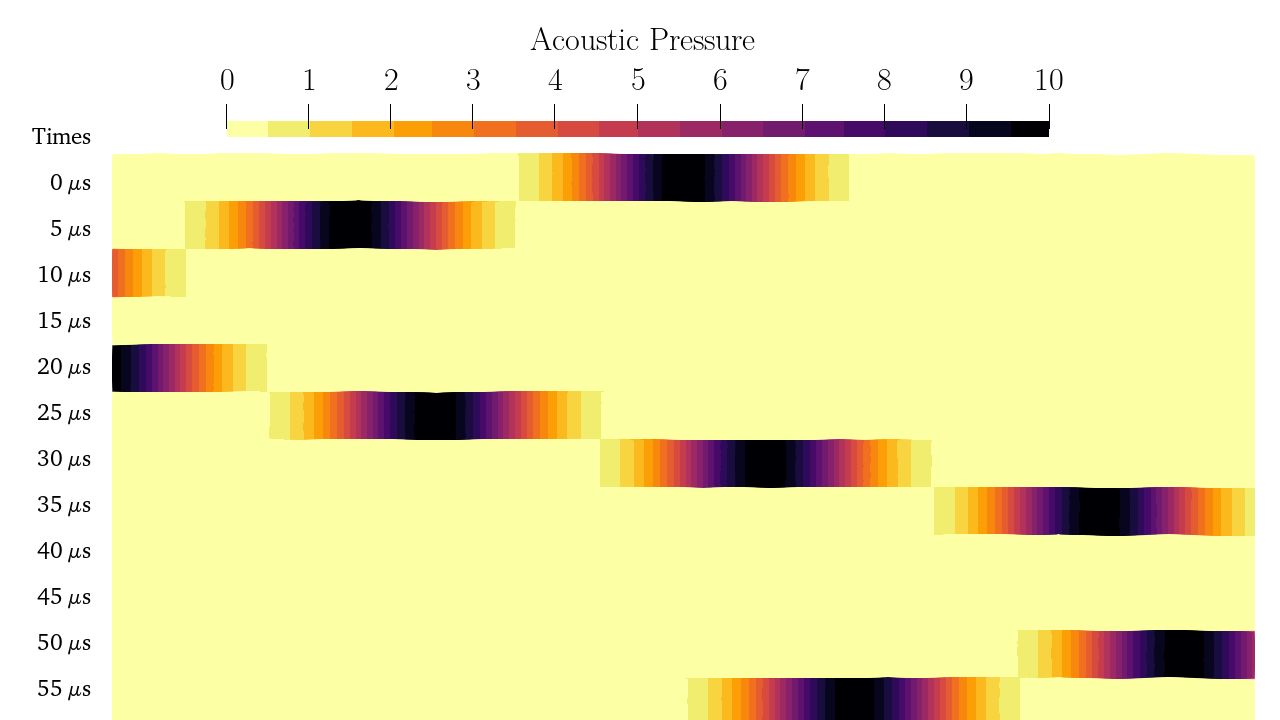
\includegraphics[scale=0.36]{assets/graphs/AC_BUMP_first_bounces_comp.png}
\caption{Acoustic pressure fields in the first 55 {\textmu}s in the DNS region in Pa. Only the top half of each DNS region is shown for comparison.}
\label{fig:ac-bump-dns}
\end{figure}

\begin{figure}[t]
\centering
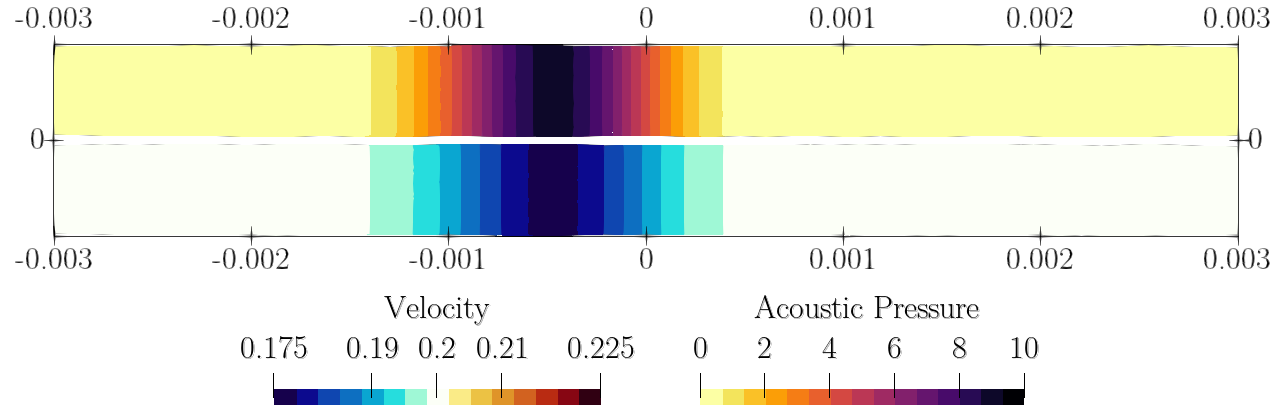
\includegraphics[scale=0.36]{assets/graphs/AC_BUMP_ndt=150e-4_comp.png}
\caption{$p_a$ and $u$ fields after 750 {\textmu}s in Pa and m s$^{-1}$. Here $u_a < 0$ so the acoustic is travelling left.}
\label{fig:ac-bump-dns-late}
\end{figure}

%% NOTE THE NON-REFLECTION IN THE DNS REGION BEFORE BOUNCES!!!!

Pressure fields for the first bounces off the up- and downstream acoustic boundary are shown in \fig{fig:ac-bump-dns}. It seems after a single bounce off each end that the ADCBCs are adequately sampling and reintroducing the acoustic bump with negligible changes to its shape. The sample rate means that roughly $(d / c) / δt_{\rm{sample}} \approx 23$ samples are used to sample the first standard deviation of width of the Gaussian. This reconstruction of acoustic shape is impressive given the lack of interpolation (\nth{0} order interpolation means using constant sample values) used. After 750 {\textmu}s, the acoustic should have been sampled by the ADCBCs and reentered the DNS domain 13 times through each boundary. Note that up to this point in the simulation, the boundary conditions have taken up less than one percent of the overall simulation runtime. This is unsurprising given how few boundary nodes there are and since the bulk of the simulation time is spent calculating gradients at the other $\sim$1000 discretisation points. The pressure and velocity fields are shown in the DNS region at this time in \fig{fig:ac-bump-dns-late}. We can see that the size of highest acoustic pressure region has shrunk somewhat so some acoustic losses have been encountered. We note here that a better test of the ADCBCs would be to compare these results against a fully simulated 1 cm long tube with hard inflows and outflows given by specifying $u=0.2$ m s$^{-1}$ at these boundaries to model the closed boundaries. This analysis is not performed in this report. Regardless, it seems as though changes to the acoustic's shape are minimal despite the short acoustic length scale. Thus, from the previous chapter we know that this error should be minimised even farther when a longer tube is simulated. For example, if a 1 m long tube is simulated instead, we expect the same error to occur at roughly $t_C = (1~\text{m} / 1~\text{cm})^2 \cross 750~\text{{\textmu}m} = 7.5$ s in the longer simulation. This should be ample time to simulate a thermoacoustically unstable flame.

\begin{figure}[t]
\centering
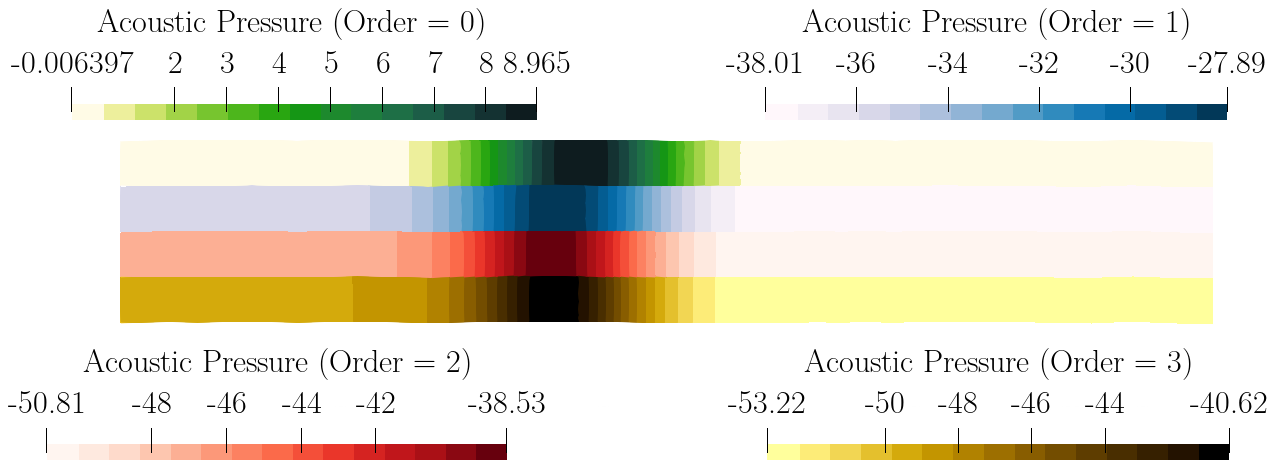
\includegraphics[scale=0.36]{assets/graphs/AC_BUMP_orders.png}
\caption{Acoustic pressures of the acoustic disturbance after 750 {\textmu}s for zero to third order interpolation (top to bottom) in Pa. Only the top half of each DNS region is shown for comparison.}
\label{fig:ac-bump-dns-orders}
\end{figure}

The above results are found provided constant interpolation is used to evaluate $\overline{\cl{L}}(t - τ)$ values. Results of the same Gaussian acoustic bump after 750 {\textmu}s for orders zero to three are shown in \fig{fig:ac-bump-dns-orders}. Bizarrely, when higher orders of interpolation are used the results massively deteriorate and large amounts of error are introduced each every bounce. After the thirteen bounces, we are left with an acoustic bump of roughly the same size $\max(p_a) - \min(p_a) \approx 10$ Pa, but with a drift in pressure much larger than this. Clearly this pressure drift is the result of the pressure difference between the front and back of the bump adding up after repeated bounces, which is most likely caused by the sampling error introduced in the previous chapter since the boundary averaging procedure should be having little to no effect in this quasi-one-dimensional test case. Although, it is unclear why this happens only when non-constant interpolation is used. Assuming it isn't the result of a mistake in the ADCBCs implementation into the SUNSET code, there is potentially some term in the error of the reintegrated acoustic upon reentry which is cancelled out when constant sample values are used, but not for interpolated values. Either way, this needs to be investigated further.

\begin{figure}[t]
\centering
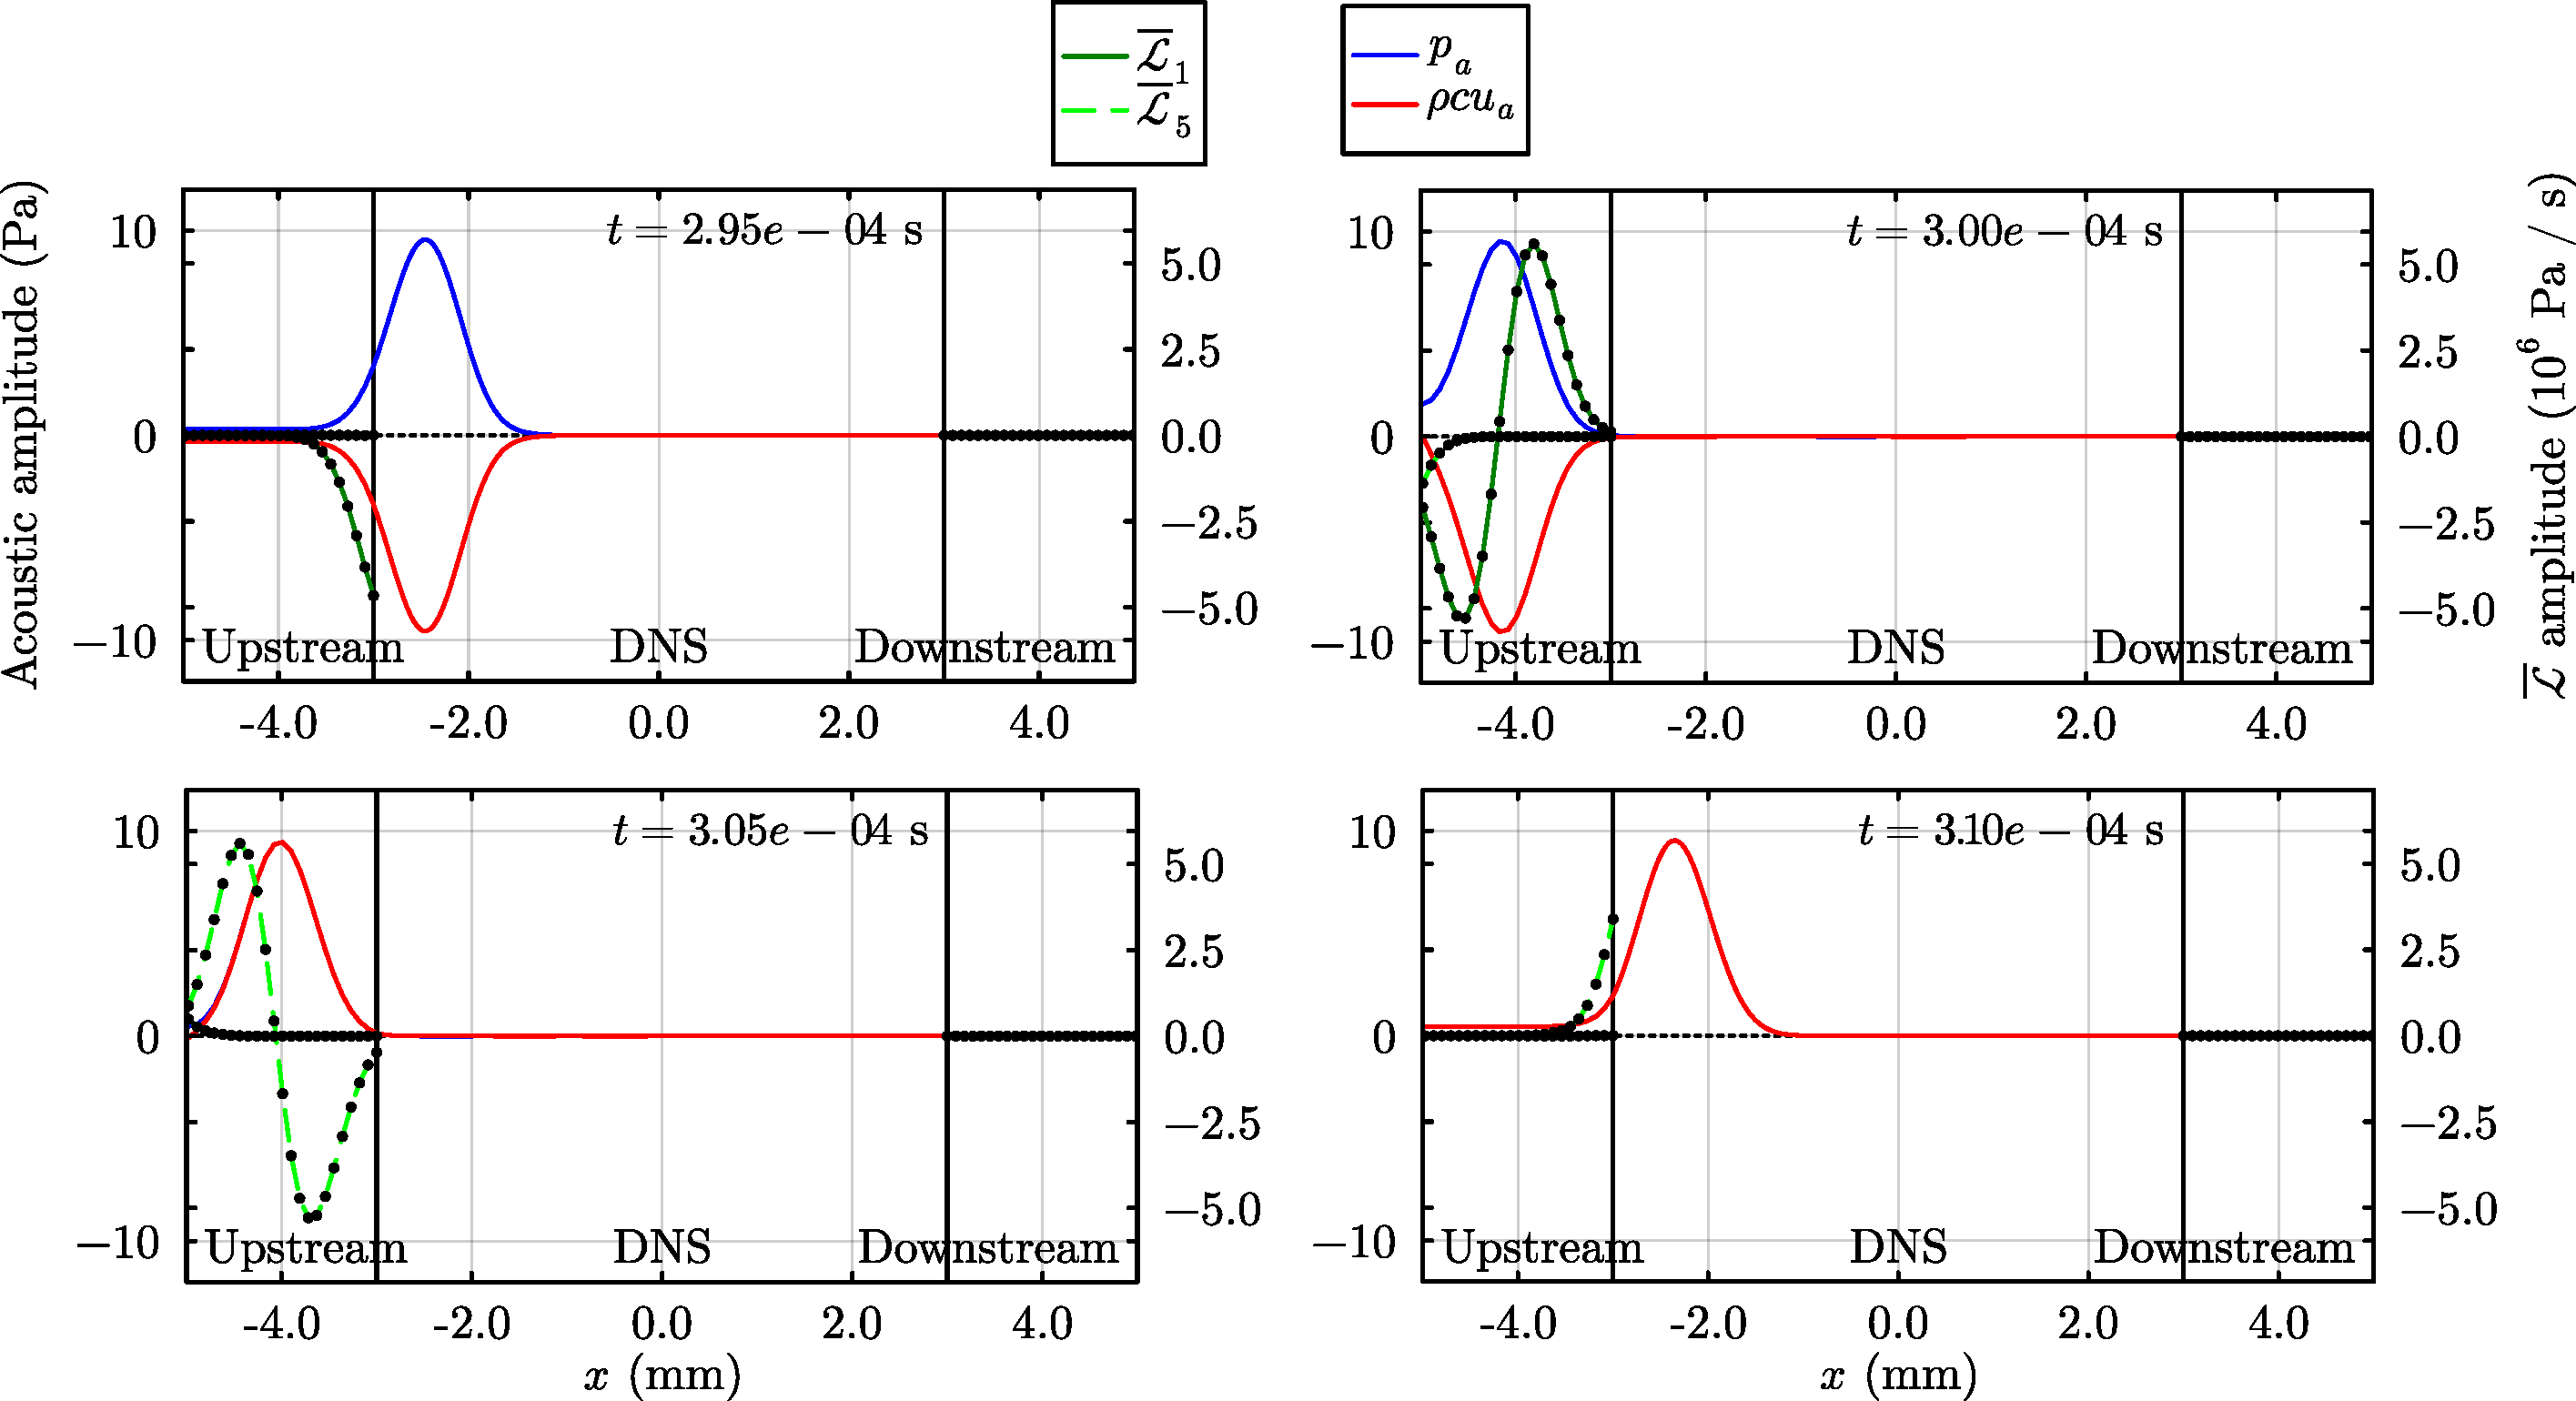
\includegraphics[scale=0.35]{assets/graphs/ac_frames_order=0.pdf}
\caption{Reconstruction of the acoustic fields in the acoustic and DNS regions for the simulation using zeroth order interpolated samples.}
\label{fig:ac-reconstruct_order0}
\end{figure}

\begin{figure}[t]
\centering
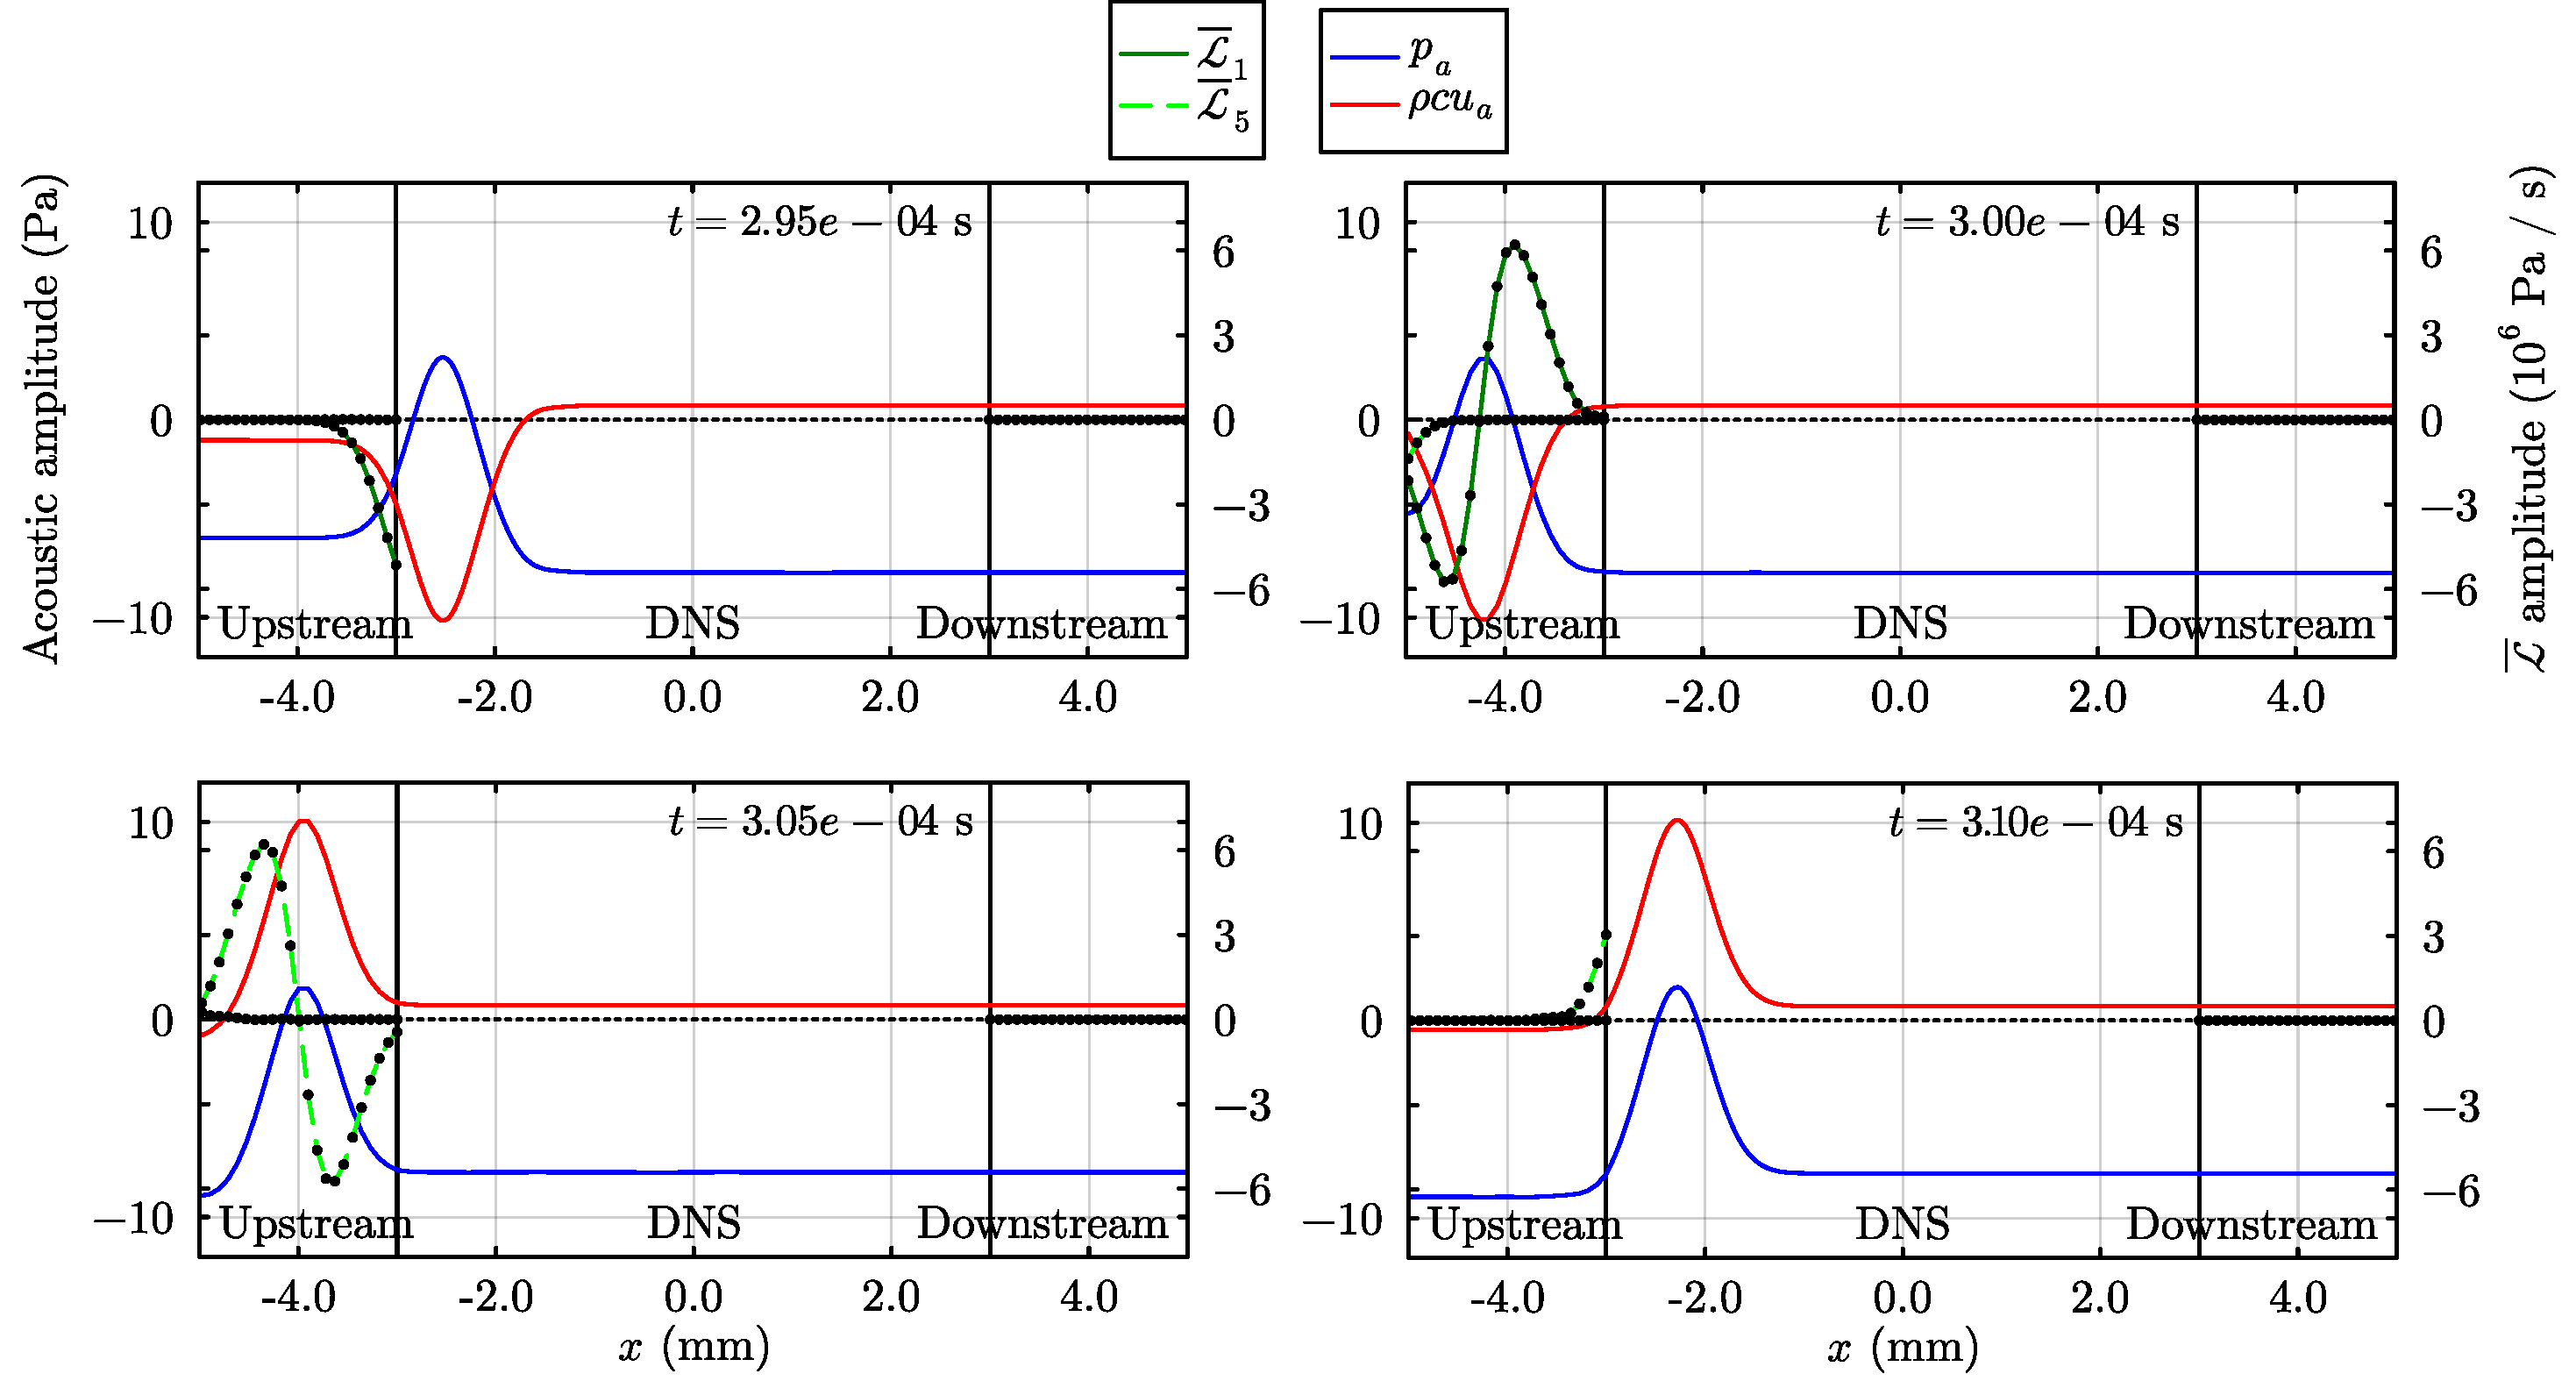
\includegraphics[scale=0.35]{assets/graphs/ac_frames.pdf}
\caption{Reconstruction of the acoustic fields in the acoustic and DNS regions for the simulation using third order interpolated samples.}
\label{fig:ac-reconstruct_order3}
\end{figure}

We can now use the discretised acoustic region field reconstruction from the previous chapter to observe the acoustics in the fictitious region in a way which is not immediately available to us from the interior DNS data. In \fig{fig:ac-reconstruct_order0} are the results for the constant interpolation, where we see although the acoustic field has dissipated by $\sim$1 Pa, the symmetric Gaussian structure is maintained. Instead, in \fig{fig:ac-reconstruct_order3} an asymmetric structure resulting in the pressure drift mentioned above. The values of $\cl{L}$ in both figures showcase these values moving with $p_a$ and $u_a$ in the upstream acoustic domain, which is roughly $\propto ζ \exp(-ζ^2)$ for some variable $ζ(t, x)$. Notice that because $R_{\rm{U}} = 1$ in both cases we get that $\cl{L}_{5, \rm{U}}(t, x_{\rm{IN}} - l_{\rm{U}}) = \cl{L}_{1, \rm{U}}(t, x_{\rm{IN}} - l_{\rm{U}})$. This should always result in the Dirichlet condition $u_a(t, x_{\rm{IN}} - l_{\rm{U}}) = 0$ and Von Neumann condition $\partial p_a / \partial x(t, x_{\rm{IN}} - l_{\rm{U}}) = 0$, although we notice that this is not true for the third order simulation. In the case where an open acoustic boundary $R_{\rm{U}} = -1$ is used instead, we have $\cl{L}_{5, \rm{U}}(t, x_{\rm{IN}} - l_{\rm{U}}) = -\cl{L}_{1, \rm{U}}(t, x_{\rm{IN}} - l_{\rm{U}})$ so the boundary conditions on $p_a$ and $u_a$ swap. Both these cases match the desired acoustic properties for open and closed tubes under typical acoustic modelling.




\section{Acoustic Standing Wave}

\begin{figure}[t]
\centering
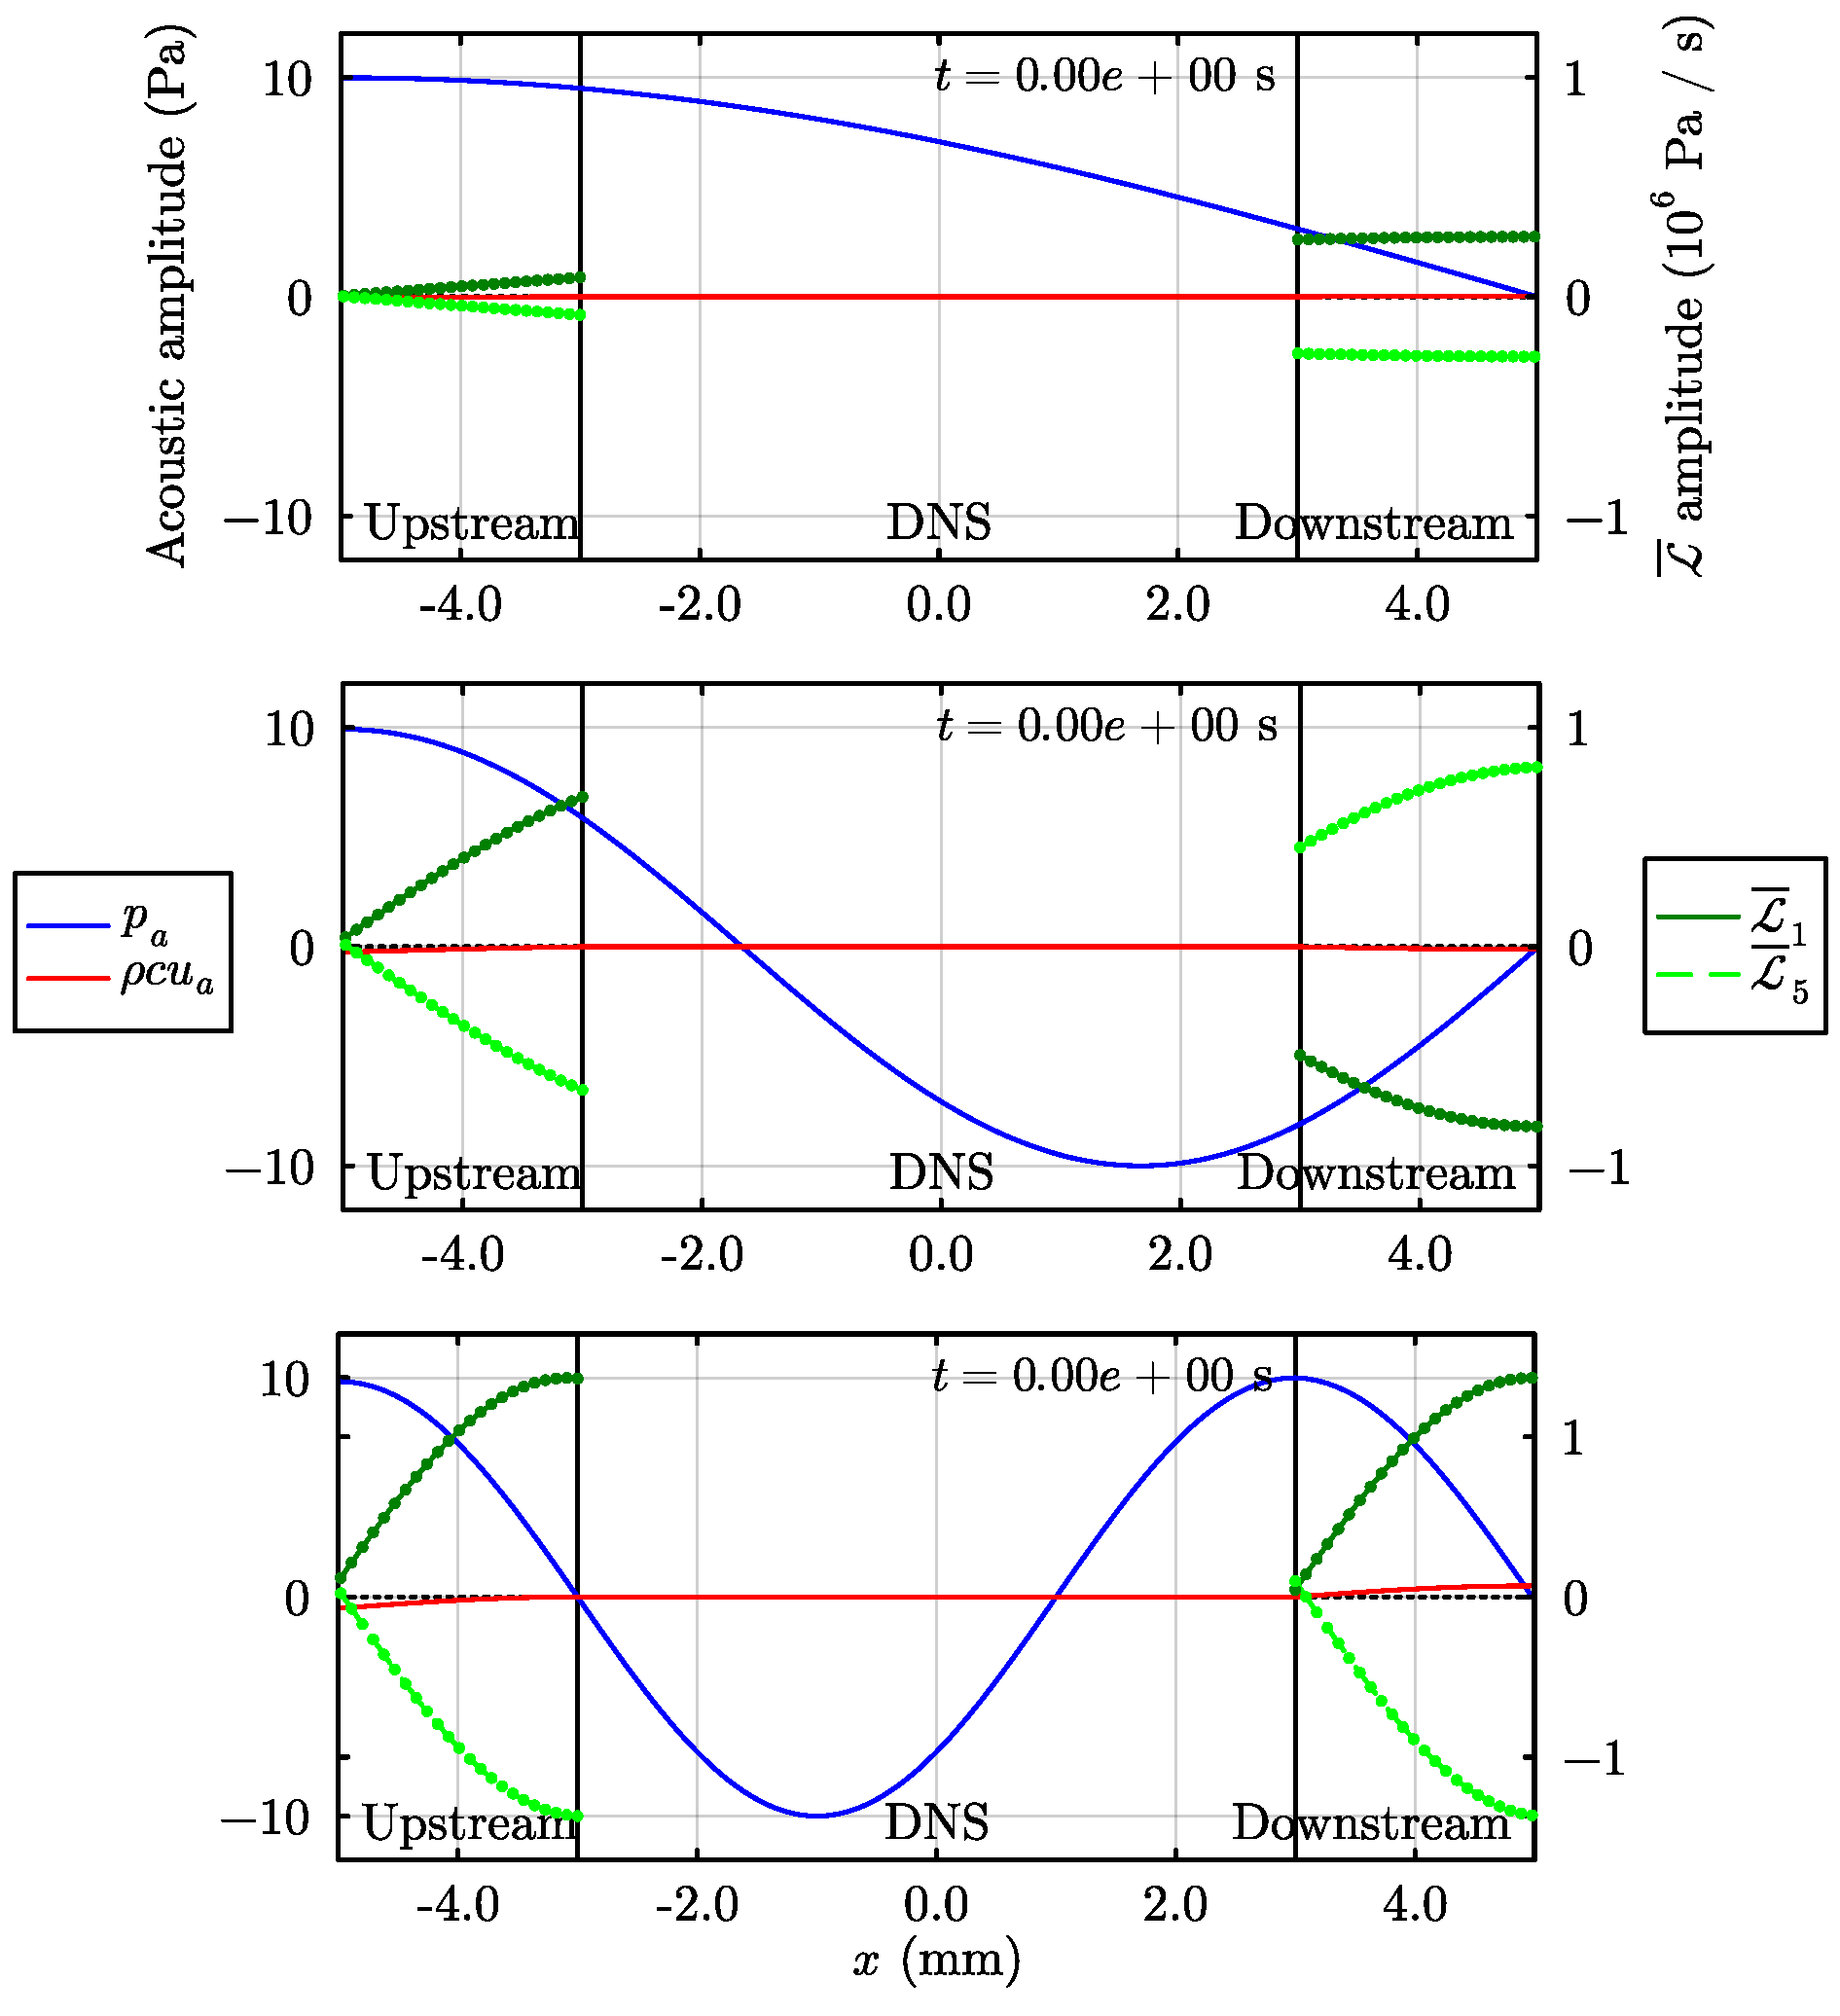
\includegraphics[scale=0.35]{assets/graphs/ac-plot-wave-modes.pdf}
\caption{Reconstruction of the initial acoustic fields for $N_κ = 1, 2, 3$.}
\label{fig:ac-wave-modes}
\end{figure}

\begin{figure}[t]
\centering
\begin{subfigure}{0.99\textwidth}
\centering
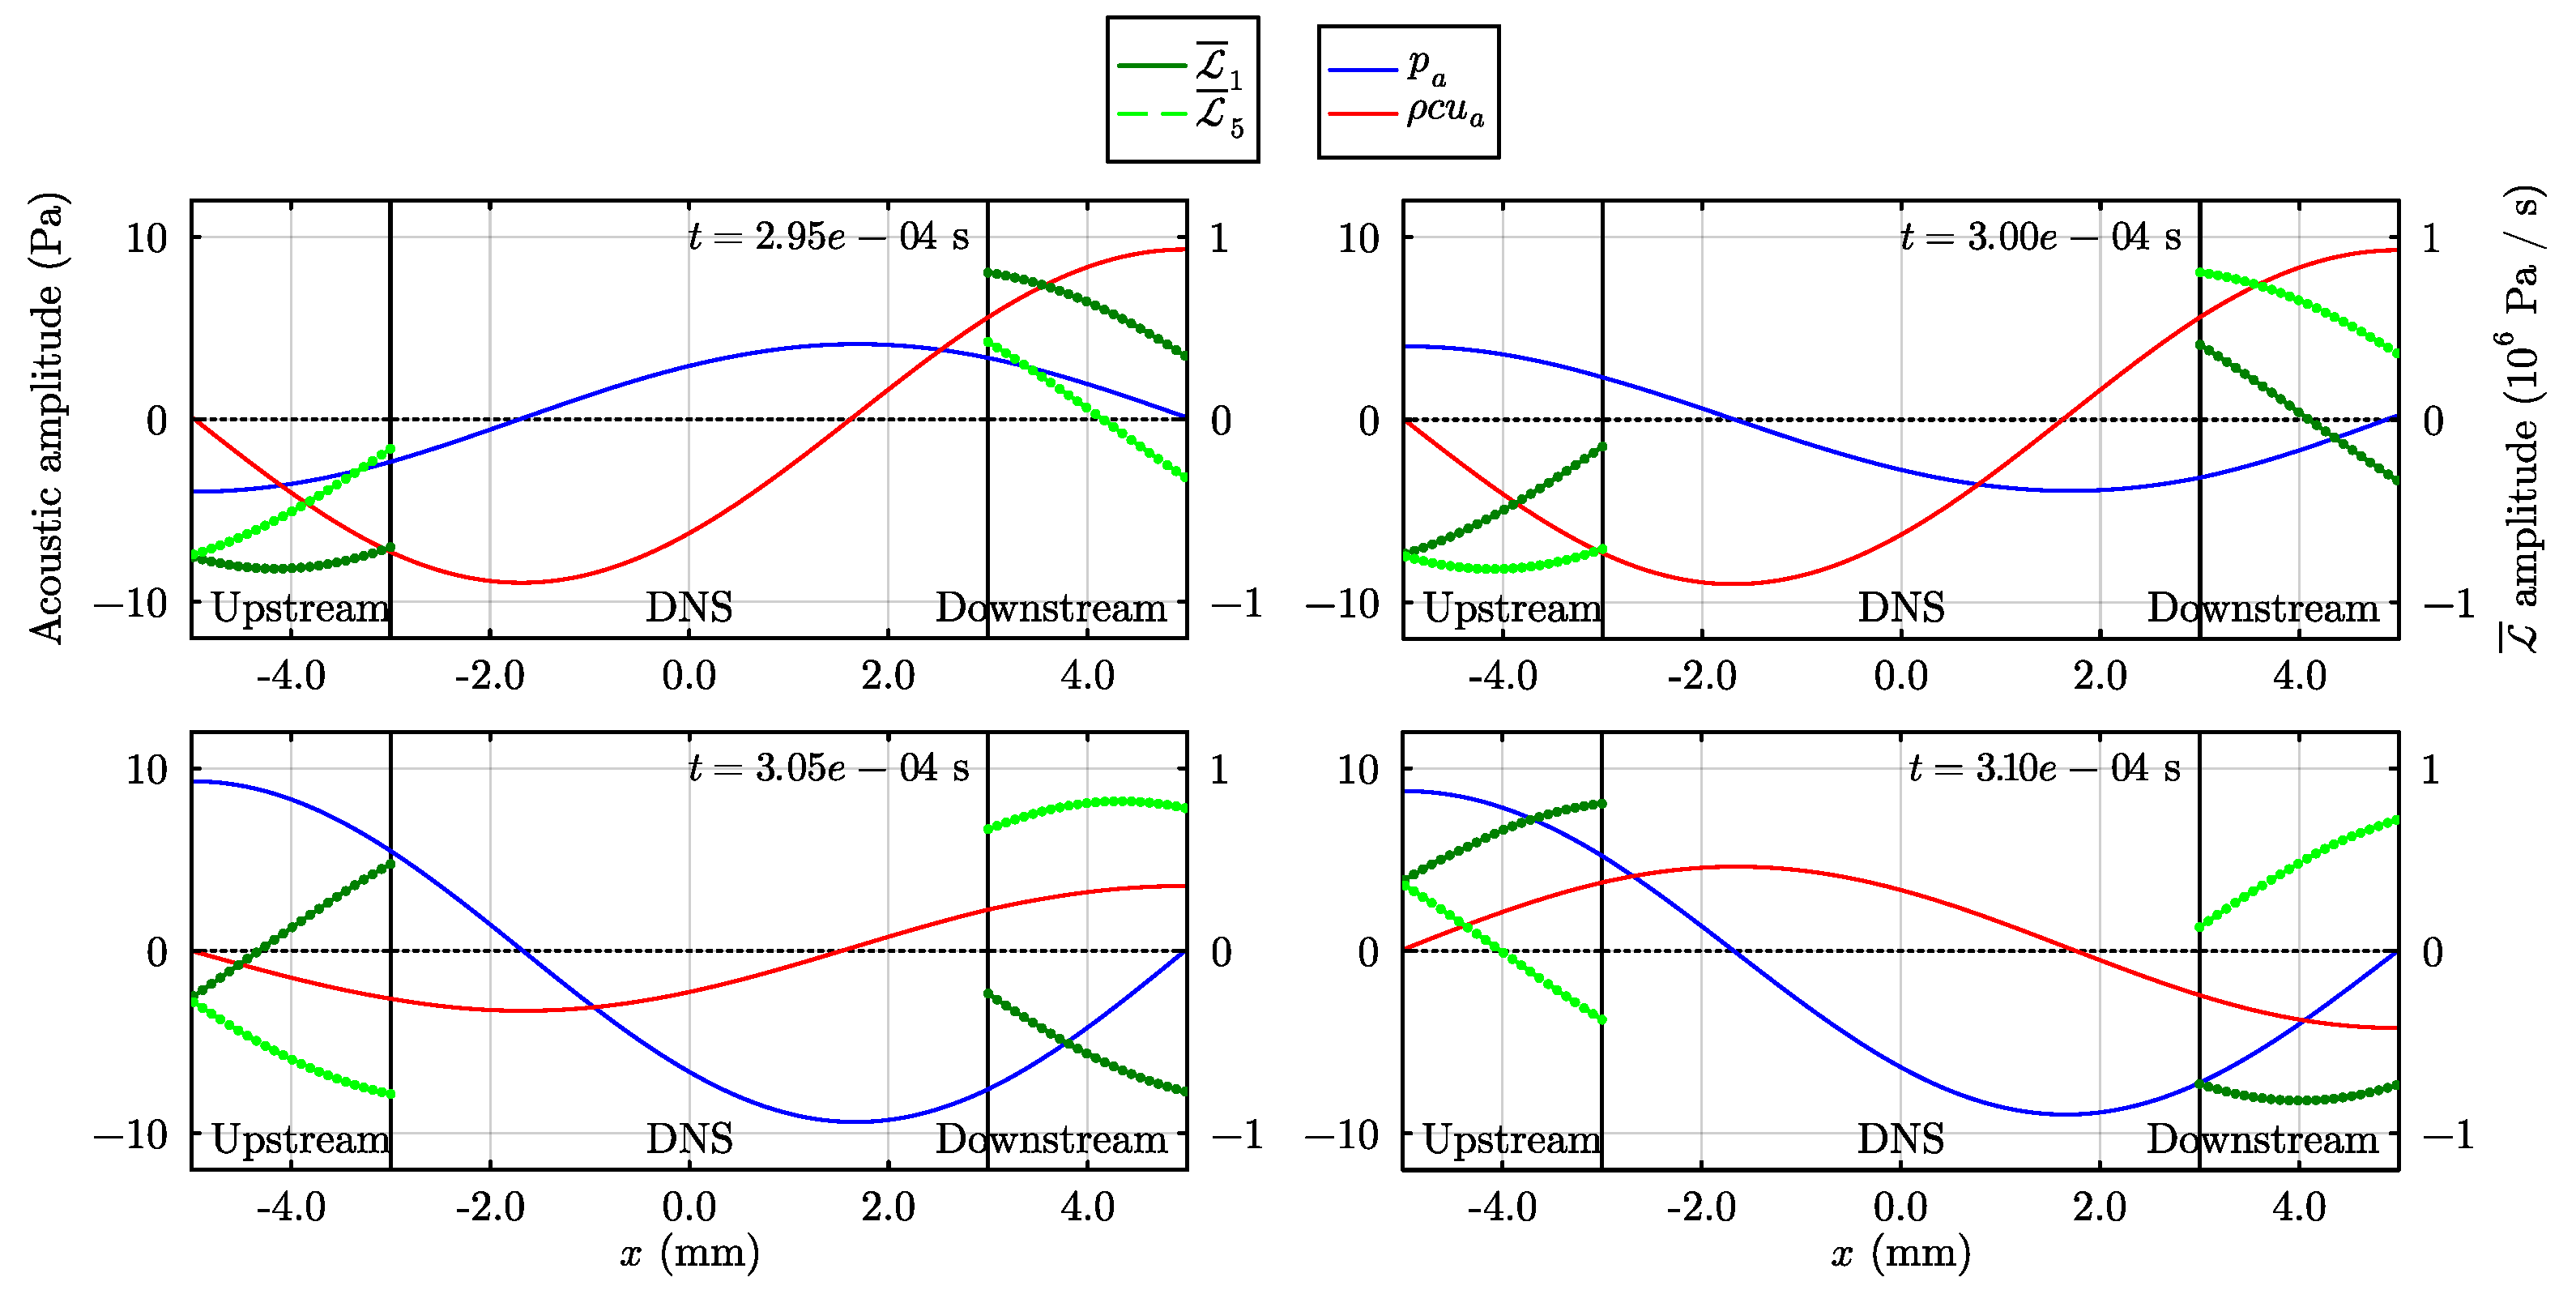
\includegraphics[scale=0.33]{assets/graphs/ac-plot-3-4_long.pdf}
\caption{Reconstruction of acoustic fields for $N_κ = 2$.}
\label{fig:ac-wave-later}
\end{subfigure}

\vspace*{0.5em}

\begin{subfigure}{0.99\textwidth}
\centering
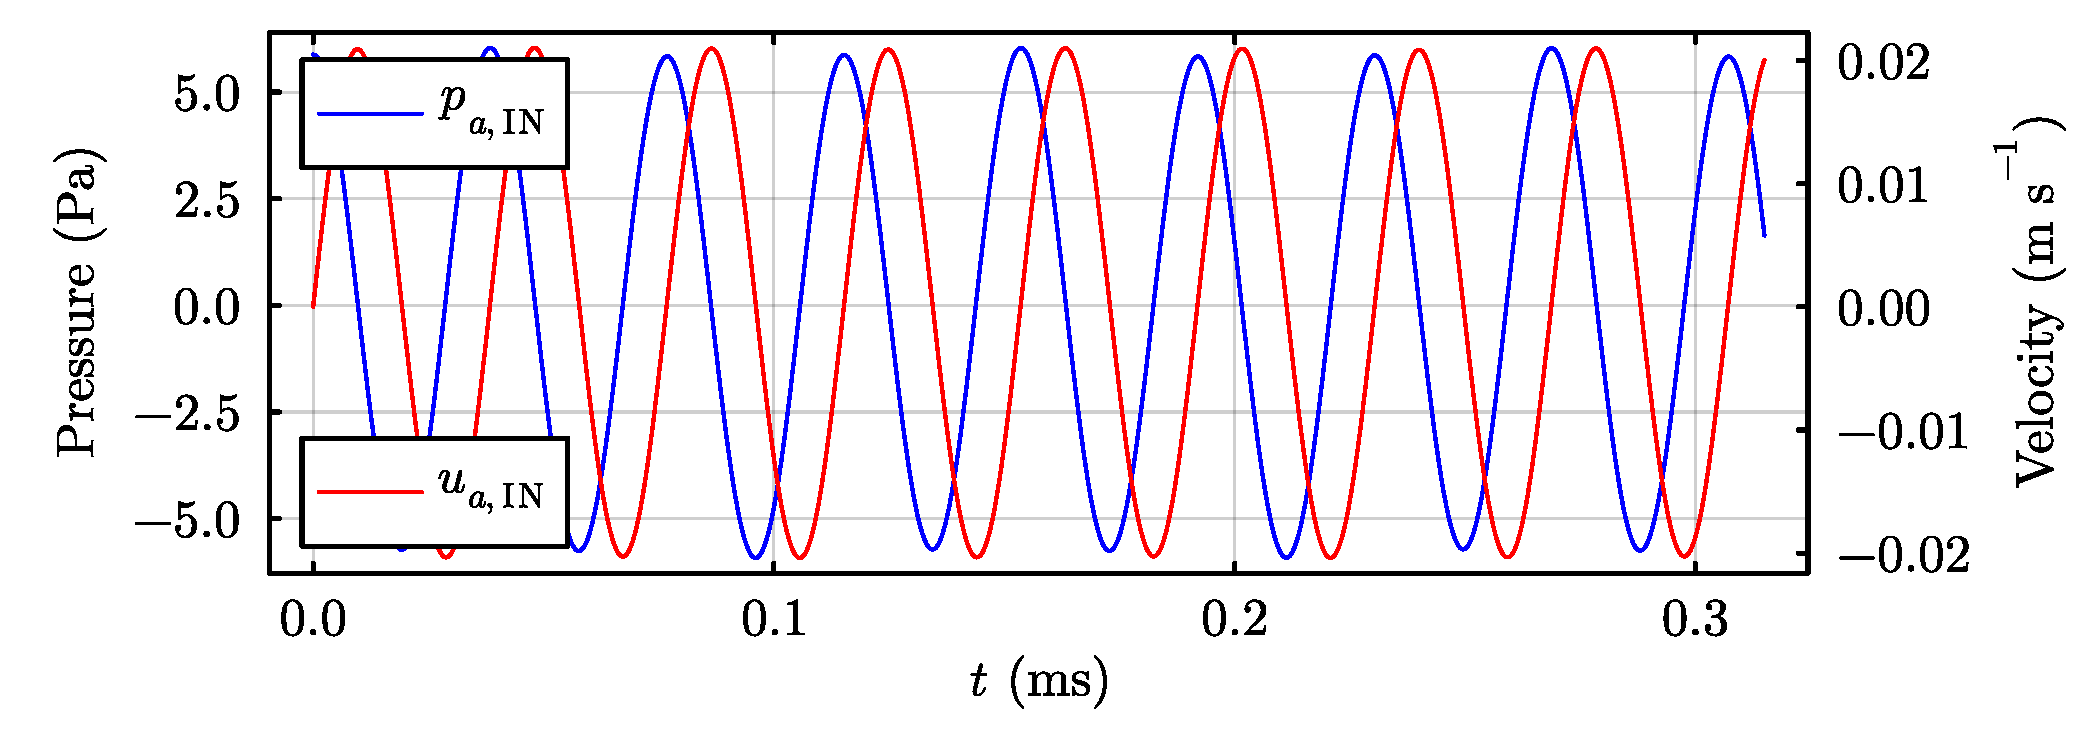
\includegraphics[scale=0.35]{assets/graphs/up_plot_wave.pdf}
\caption{Time series of acoustic pressure and velocity at the ADCBC inflow for $N_κ = 2$.}
\label{fig:up_plot_wave}
\end{subfigure}
\caption{}
\label{fig:wave-later}
\end{figure}

We now initialise an acoustic standing wave in the same computational domain as the previous test case, using the same fluid properties and ADCBC parameters, except for the change that we instead model an open upstream acoustic boundary, so $R_{\rm{D}} = -1$ instead and we use constant interpolation. The desired initial acoustic pressure is:
\begin{equation}
p_A(t = 0, x) = A \cos\left( 2 π \, \frac{x - x_{\rm{IN}} - l_{\rm{U}}}{l_{\rm{tube}}}  \, \frac{2N_κ - 1}{4}\right),
\end{equation}
where $A = 10$ Pa is the acoustic amplitude as before and $l_{\rm{tube}} \equiv l_{\rm{U}} + (x_{\rm{OUT}} - x_{\rm{IN}}) + l_{\rm{D}}$ is the full tube length with $l_{\rm{U}} = l_{\rm{D}} = 2$ mm and $(x_{\rm{OUT}} - x_{\rm{IN}}) = 6$ mm. $N_κ$ determines the wavenumber of the standing wave: if $N_κ = 1$ we have the $1 / 4$ mode, if $N_κ = 2$ we have the $3 / 4$ mode etc.. The corresponding wavenumber is:
\begin{equation}
κ = \frac{2N_κ - 1}{4 l_{\rm{tube}}}
\end{equation}
In the DNS region, the wave can be initialised by directly calculating $p_a(0, x)$ values. In the upstream and downstream region, however, we must instead calculate $\cl{L}_{1/5}(t = 0, x)$ using the formulae in \equ{eqn:λ_l_L}, discretise them and enter the resulting finite values into the initial queues $(\bb{T} \cross \bb{L})(t = 0)$ for the ADCBC inflow and outflow. The same LABFM discretisation is used as the acoustic bump test case above. \fig{fig:ac-wave-modes} shows the acoustic initial conditions in the full tube for the first three standing wave modes. In each of the three graphs, the wave continues smoothly into the acoustic domain owing the acoustic reconstruction introduced in the previous chapter. \fig{fig:ac-wave-later} shows the simulation after a few acoustic periods for the $N_κ = 2$ case. Clearly $u_a(t, x_{\rm{IN}} - l_{\rm{U}}) = 0$ and $p_a(t, x_{\rm{OUT}} + l_{\rm{D}}) = 0$ as desired. In this case you can see the reconstructed $\cl{L}_{1/5}$ fields travelling left and right respectively. Note that in the $N_κ = 2$ and 3 modes you can see a slight error with some $u_a(t = 0, x) \ne$ values in the up and downstream domain due to inaccuracies with the post-processing code. In \fig{fig:up_plot_wave} we have a time series of $p_{a}$ and $u_{a}$ values at the inflow boundary. Note that the maximum amplitude the waves reach at this inflow boundary is $\sim$6 Pa, hence the lower amplitude.

\begin{figure}[t]
\centering
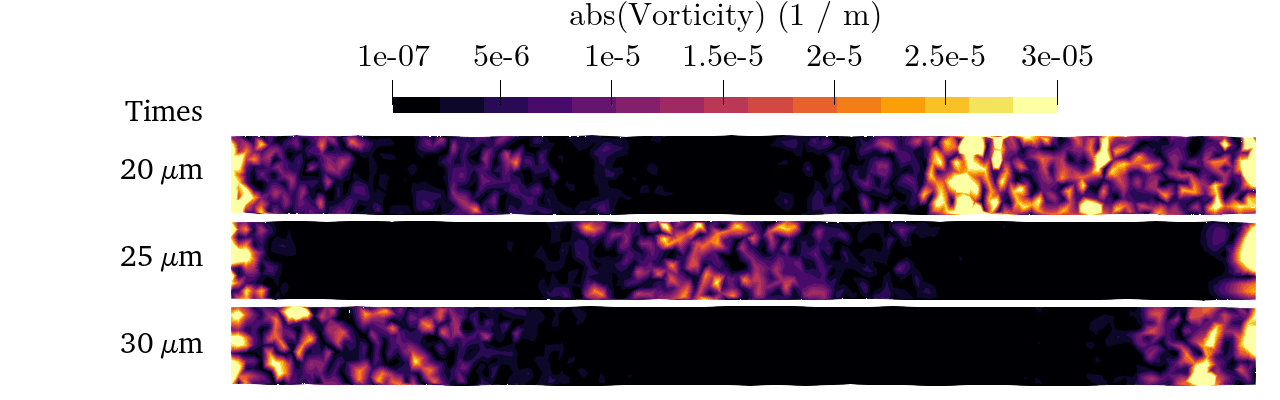
\includegraphics[scale=0.36]{assets/graphs/AC_WAVE_QWAVE.png}
\caption{Spurious vorticity wave travelling through the DNS domain at the acoustic speed for the $N_κ = 2$ wave.}
\label{fig:vort-wave}
\end{figure}

Focusing instead on the DNS region, looking only at vorticity disturbances -- given that the background vorticity should be $\vb{ω} \equiv \vb{\nabla}\cross\vb{u} \equiv 0$ for the one-dimensional flow -- we can see in \fig{fig:vort-wave} a vorticity perturbation travelling at the acoustic speed, right to left. This can also be seen in disturbances to $v$. Not depicted in the figure is this wave and another bouncing back and forth through the DNS domain, as if it is being transmitted through the full acoustic domain. This is likely the result of the coupling of $x$ and $y$ velocities in the momentum equation introducing $\cl{O}(h^{k - 2 + 1}) = \cl{O}(h^{k_{\rm{HV}} - 4 + 1}) = \cl{O}(h^{3})$ discretisation error, which is largest at the peaks of the acoustic wave. Note also the larger values of $\abs{\vb{ω}}$ at the characteristic boundaries. most likely due to variations of $u$ and $\cl{L}_{1/5, \rm{nonreflect}}$ along the boundary resulting from similarly sized discretisation error.

Eventually, due to the sampling error introduced as the wave continuously enters the two ADCBC boundaries we expect in this small domain for wave to dissipate. Although this seems to take enough time that, yet again, for longer modelled tubes this effect should be unimportant.

% We use SI units (1 / m)
\begin{figure}[t]
\centering
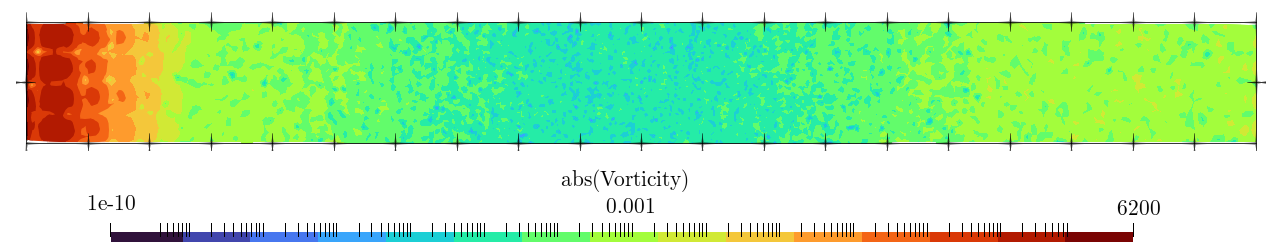
\includegraphics[scale=0.36]{assets/graphs/u-inflow-instab.png}
\caption{The wringing inflow instability, shown with a logarithmic plot of vorticity magnitude in inverse metres.}
\label{fig:inflow-instab}
\end{figure}

Under certain boundary discretisation schemes, a wringing instability in $u$ was observed at the inflow after many acoustic periods. This grows exponentially, suggesting that the instability behaves linearly, until the vorticity produced within the inflow region destroys the solution. This wringing behaviour is shown at a late stage of instability in \fig{fig:inflow-instab}. In this figure, four distinct cells of high vorticity are seen along the boundary, suggesting two wavelengths of the unstable mode fit in the vertical width of the symmetric domain. For the boundary discretisations this instability occurred with, it only occurred at the inflow what ADCBC inflows and outflows were used, suggesting it needs a continuous source of acoustics entering the upstream acoustic region. This instability was successfully inhibited in the other simulations by using a more stable boundary discretisation. Before this improved boundary discretisation was found, the instability was treated by simply increasing amplitude of the tangential hyperviscosity filter at the boundary nodes, so that the wringing mode was suppressed. The cause of the instability was likely the boundary averaging procedure coupling with the boundary discretisation, resulting in a feedback loop exacerbating tangential $u$ deviations. Hence, it seems reasonable that this instability should be precluded in an ADCBC formulation which does not perform boundary averaging, although this needs to be properly investigated.

\begin{figure}[t]
\centering
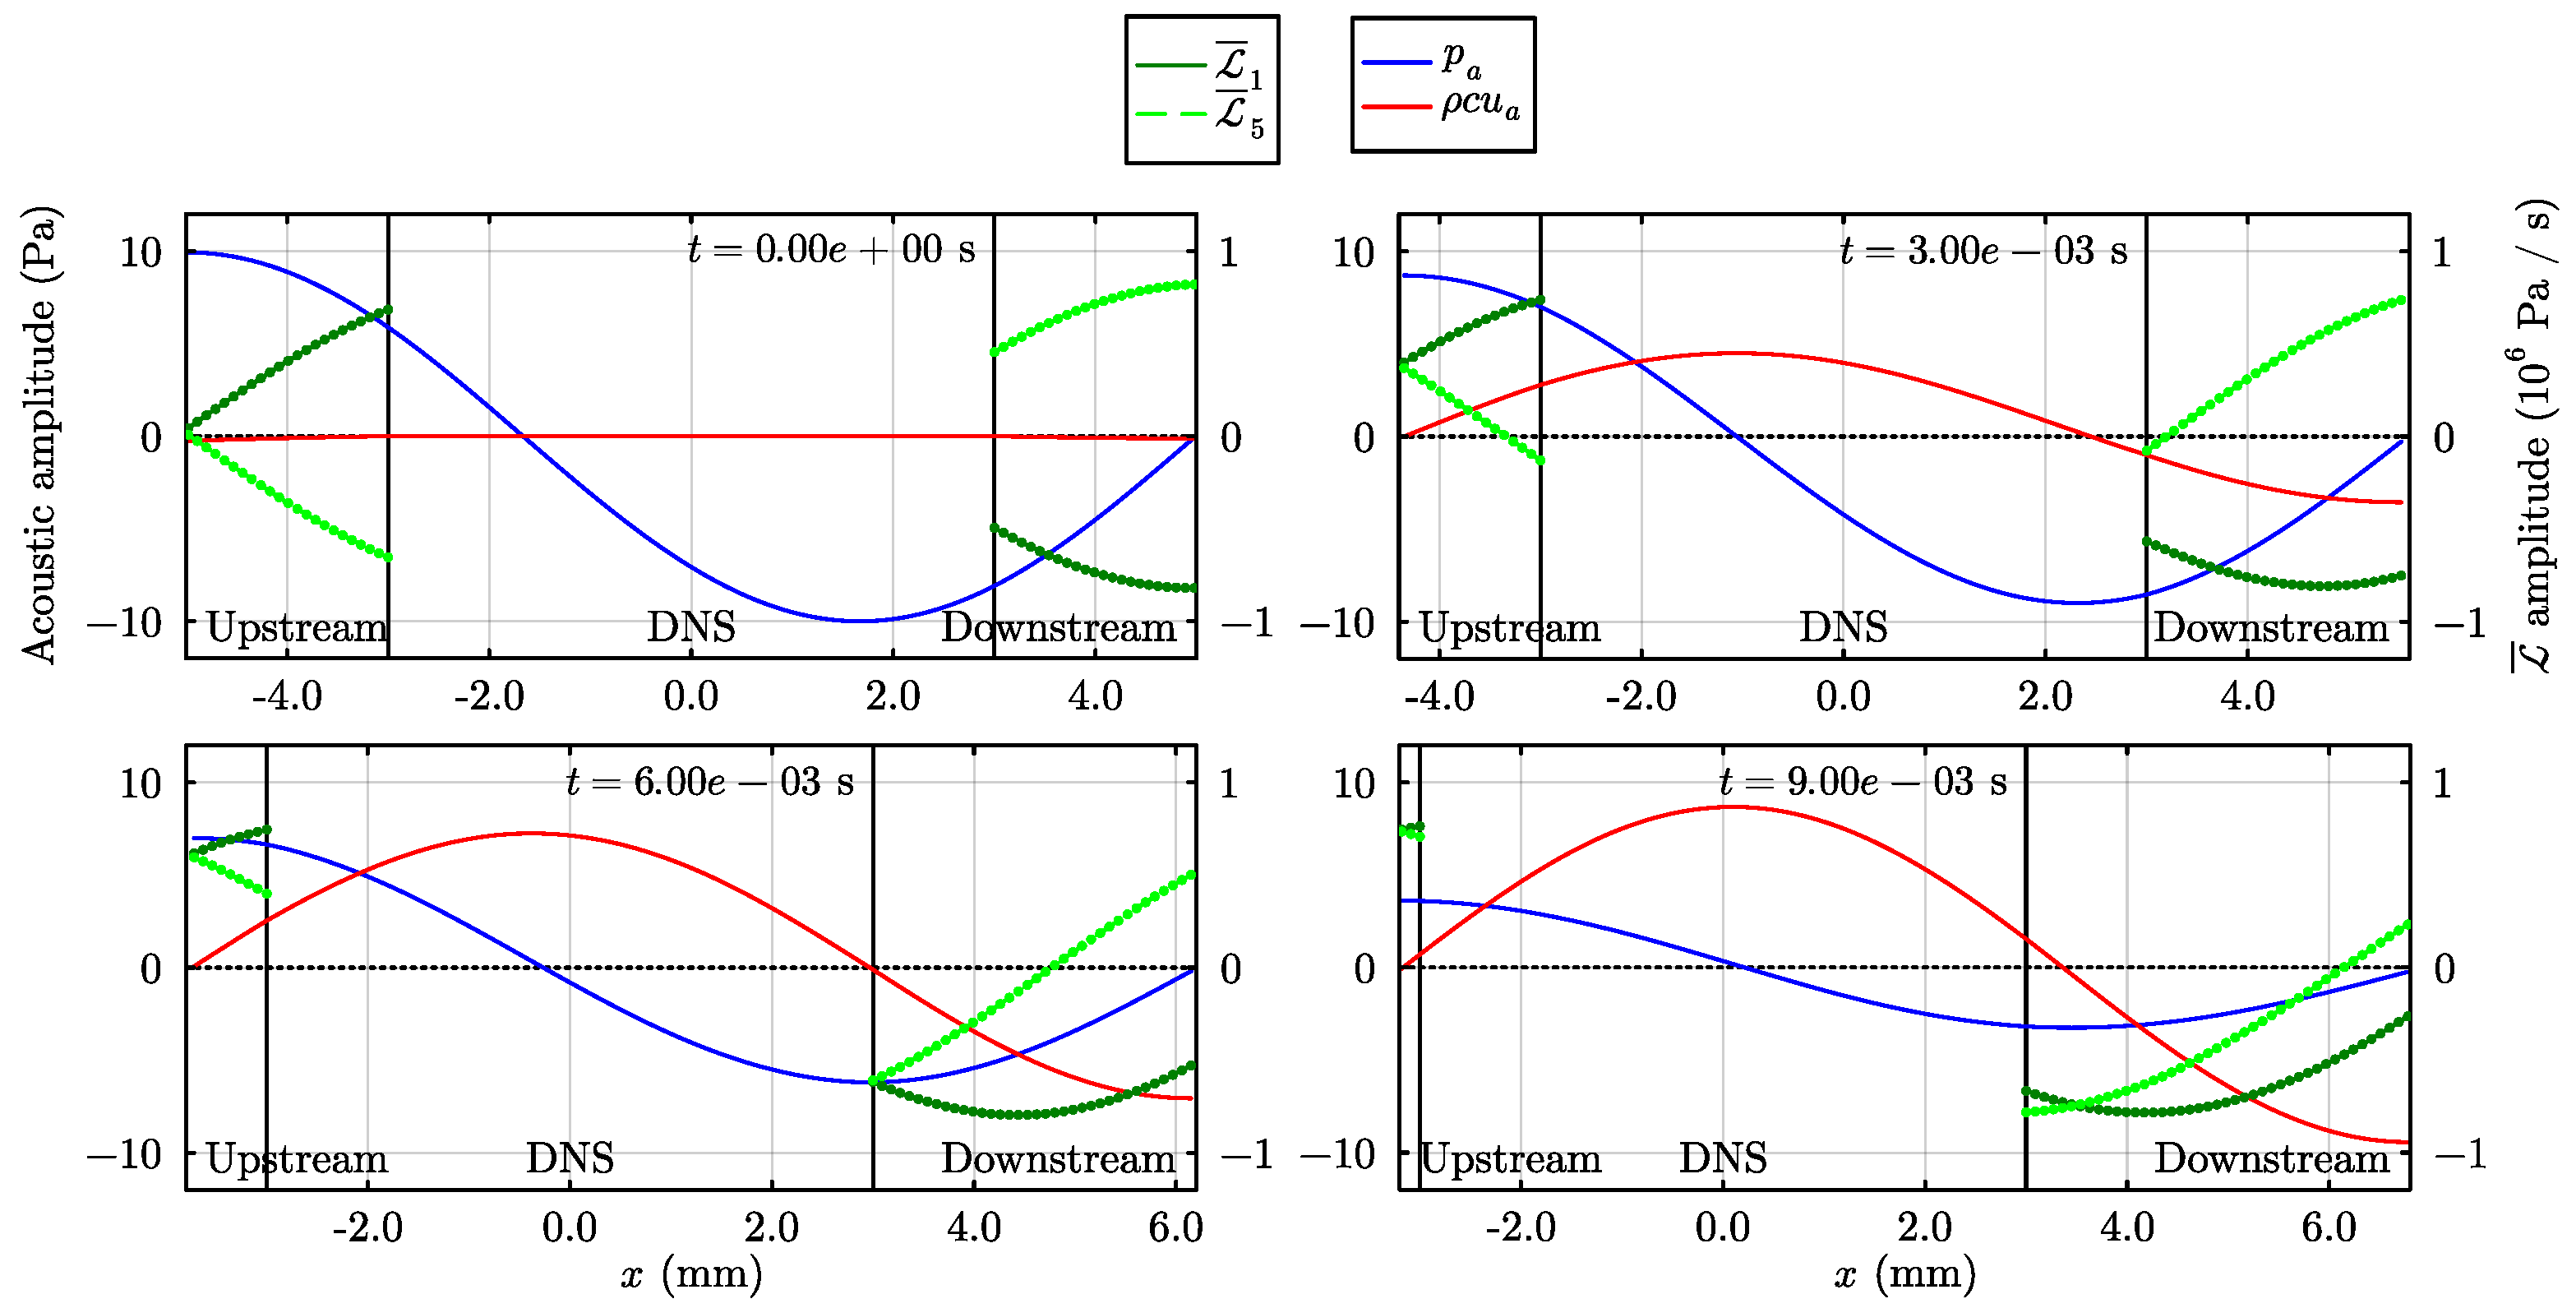
\includegraphics[scale=0.33]{assets/graphs/ac-plot-3-4_moving.pdf}
\caption{Simulation of the $N_κ = 2$ standing wave using changing delay times to simulate a translating DNS region over a longer period of time.}
\label{fig:moving-dns-region}
\end{figure}

Now we test the ability of the ADCBCs to successfully model a DNS domain which is being translated along the acoustic domain. In doing so, we hope to justify using the left-to-right flow to stabilise a flame inside the domain by allowing the DNS domain to move right-to-left in the acoustic domain to compensate. Mathematically, we do this simply by updating the upstream and downstream time delays regularly such that:
\begin{equation}
τ_{\rm{U}}(t) = \frac{2}{c} (l_{\rm{U}, 0} - \overline{u}_{\rm{in}} t)
\quad \text{and} \quad
τ_{\rm{D}}(t) = \frac{2}{c} (l_{\rm{D}, 0} + \overline{u}_{\rm{in}} t),
\end{equation}
where $l_{\rm{U/D}, 0}$ are the initial up- and downstream acoustic region lengths and $\overline{u}_{\rm{in}}$ is the non-acoustic inflow velocity. In later simulations, if the non-acoustic inflow velocity is changing (e.g. to stabilise a thermoacoustic flame), we would instead use:
\begin{equation}
δτ_{\rm{U}}(t^n) = - \frac{2 \overline{u}_{\rm{in}}(t^n)}{c} δt^n
\quad \text{and} \quad
δτ_{\rm{D}}(t^n) = \frac{2 \overline{u}_{\rm{in}}(t^n)}{c} δt^n,
\end{equation}
where $t^n$ is the new simulation time, $δt^n$ is the time step size and $τ_{\rm{U/D}}(t^n) = τ_{\rm{U/D}}(t^{n - 1}) + δτ_{\rm{U/D}}(t^n)$. This is essentially a forward Euler integration, which will be accurate enough provided the non-acoustic inflow velocity is slowly-varying enough. Regardless, \fig{fig:moving-dns-region} shows these changing delay times being used in a longer simulation of the same 3/4 mode standing wave. Despite the translated DNS region in the latter three graphs, the acoustic mode remains the same (albeit with a change in phase). Note that the accuracy of the wave in the later graphs justifies the previous use of the low Mach number approximation: despite the use of non-convected waves to model the time delay (and field reconstruction), the wave remains accurately resolved.

% With the correct frequency???




\section{Thermoacoustically Unstable Flame}

\subsection{Acoustic Eigenmodes}

Before simulating a thermoacoustically unstable flame using the ADCBCs, we first need to find the acoustic eigenmodes of the closed-open tube with a density discontinuity in the middle. Unlike the tube without a density discontinuity, we expect acoustics which meet the flame not to be fully transmitted over, but partially transmitted and partially reflected. In this sense, we must instead model the tube using boundary conditions which corroborate this. To the left and right of the flame, the fully nonlinear acoustics may be described by the non-dimensional equations:
\begin{subequations}
\begin{alignat}{4}
  & \pdv{ρ}{t} + \Ma &        & \pdv{ρ u}{x} &&= 0 \\
ρ & \pdv{u}{t} + \Ma & \, ρ u & \pdv{u}{x}   &&= -\pdv{p}{x} \\
  & \pdv{p}{t} + \Ma &      u & \pdv{p}{x}   &&= \frac{1}{\Ma} \frac{c^2}{c_{\rm{U}}^2} ρ \pdv{u}{x}
\end{alignat}
\end{subequations}
where all variables in the above equations are non-dimensional. Space is non-dimensionalised by tube length $l_{\rm{tube}}$ such that $x \in [0, 1]$, velocity by flame speed $S_L$, time by characteristic acoustic time $l_{\rm{tube}} / c_{\rm{U}}$, density by upstream density $ρ_{\rm{U}}$, pressure by upstream acoustic pressure $ρ_{\rm{U}} c_{\rm{U}} S_L$ and temperature by upstream temperature $T_{\rm{U}}$. Hence, far upstream temperatures are $T=1$ and far downstream temperatures are $T=r$ where r is the ratio of densities. By the dimensional relation $\hat{ρ} c^2 = γ \, \hat{p}$ (where hats represent dimensional variables) we have that $c_{\rm{D}}^2 = r c_{\rm{U}}^2$. The Mach number is $\Ma \equiv S_L / c_{\rm{U}}$.

Assuming acoustics of low enough amplitude, we find split our variables in steady states and their acoustic perturbations $ρ \equiv \overline{ρ} + ρ_a$, $T \equiv \overline{T} + T_a$, $u \equiv \overline{u} + u_a$, $p \equiv \overline{p} + p_a$ such that the non-linear coupling of the acoustics onto the density may be neglected. That is, $ρ_a \equiv 0$ so the acoustics are not strong enough to effect density in a way which would affect $u_a$ or $p_a$. Likewise with temperature perturbations, so $T_a \equiv 0$ and $T = \oT = c^2 / c_{\rm{U}}^2$. This results in the wave equations:
\begin{subequations} \label{eqn:wave_eqn}
\begin{align} 
\pdv[2]{u_a}{t} - \oT \pdv[2]{u_a}{x} &= 0 \label{eqn:wave_eqn_u} \\
\pdv[2]{p_a}{t} - \pdv{x} \left( \oT \pdv{p_a}{x} \right) &= 0 \label{eqn:wave_eqn_p}
\end{align}
\end{subequations}
where pressure and velocity acoustics are related by $\overline{ρ} \, \partial u_a / \partial t = \partial p_a / \partial x$ and we have made the assumption of a non-convected flow $\overline{u} \equiv 0$ and constant background pressure over the flame $\overline{p}_{\rm{U}} \equiv \overline{p}_{\rm{D}}$ which is physically reasonable for a slow flame travelling into a quiescent reactant mixture. Before introducing the discontinuity, we can close this system by introducing the boundary conditions $u_a(x = 0) = 0$ and $p_a(x = 1) = 0$ to model a closed-open tube.

We now enforce the discontinuous temperature and density profile, with the flame located at $x_f \in (0, 1)$ representing the flame location and separating the fields $\oT_{\rm{U}} = 1$, $\oT_{\rm{D}} = r$, $u_a(x_f^-) = u_{a, \rm{U}}(x_f^-)$, $u_a(x_f^+) = u_{a, \rm{D}}(x_f^+)$ and so on. The wave equations \equ{eqn:wave_eqn} now describe the propagation on either side of the flame we use the boundary conditions \cite{gaton-perez2025MitigationThermoacousticInstabilities}:
\begin{equation} \label{eqn:flame-BCs}
p_{a, \rm{U}}(x_f^-) = p_{a, \rm{D}}(x_f^+)
\quad \text{and} \quad
u_{a, \rm{U}}(x_f^-) = r \, u_{a, \rm{D}}(x_f^+).
\end{equation}
This junction also implicitly contains information on how waves are transmitted and reflected over this density jump. Note that if $r = 1$ or $x_f = 0, 1$, we end up in the situation of isothermal acoustics, which have the classical eigenmode solutions (the previous test case). To find non-isothermal eigenmodes, we use the time-harmonic factor $u_a, p_a \propto \exp(i ω t)$ where $ω \equiv ω_r + i ω_i$. The real part represents frequency and the imaginary part represents mode damping. Note that because we are not modelling any dissipative effects in this simple model, we expect $ω_i = 0$ in all cases. One can show that $u_a = i (\oT / ω) \partial p_a / \partial x$, so we only need to solve our system for $p_a$. Note that because our system is of finite length, we expect the allowed values of $ω$ to be quantised to a discrete countable set (c.f. electron in a box). The boundary value problem for $p_a$ is:
\begin{subequations}
\begin{gather}
\pdv[2]{u_a}{t} - \oT \pdv[2]{u_a}{x} = 0, \\
\pdv{p_{a, \rm{U}}}{x}\,(x = 0) = 0,
\qquad
p_{a, \rm{D}}(x = 1) = 0,
\qquad
p_{a, \rm{U}}(x_f^-) = p_{a, \rm{D}}(x_f^+),
\qquad
\pdv{p_{a, \rm{U}}}{x}\,(x_f^-) = r \pdv{p_{a, \rm{D}}}{x}\,(x_f^+).
\end{gather}
\end{subequations}
where $p_a \in \bb{C}$ alongside some appropriate initial conditions for the given eigenmode. Using the time-harmonic assumption, we define the function $φ(x) \equiv p_a(x) / \exp(i ω t) \in \bb{C}$ so the second order PDE in time and space becomes a second order ODE in space:
\begin{subequations}
\begin{gather} \label{eqn:BVP_phi}
φ'' + \frac{ω^2}{\oT} φ = 0, \\
φ_{\rm{U}}'(0)=0,
\qquad
φ_{\rm{D}}(1)=0,
\qquad
φ_{\rm{U}} (x_f^-) = φ_{\rm{D}}(x_f^+),
\qquad
r \, φ_{\rm{U}}'(x_f^-) = φ_{\rm{D}}'(x_f^+).
\end{gather}
\end{subequations}
The complementary functions of this equation are defined on either side of $x_f$ by solutions to the complex harmonic oscillator:
\begin{equation}
φ_{\rm{U/D}}(x) = a_{\rm{U/D}} \exp\left(- i \frac{ω}{\sqrt{\oT}} x\right) + b_{\rm{U/D}} \exp\left(i \frac{ω}{\sqrt{\oT}} x\right),
\end{equation}
where $a_{\rm{U/D}}, b_{\rm{U/D}} \in \bb{C}$ represent an extra four degrees of freedom for each side of each eigenmode. Because the boundary conditions for $φ$ are linear in $a_{\rm{U/D}}$ and $b_{\rm{U/D}}$, however, the problem of satisfying the boundary constraints boils down to finding the non-trivial (i.e. non-zero) solutions to the linear equation:
\begin{subequations}
\begin{equation}
\vb{0} = \begin{pmatrix}
φ_{\rm{U}}'(0) \\
φ_{\rm{D}}(1)  \\
φ_{\rm{D}}(x_f^+) - φ_{\rm{U}} (x_f^-)  \\
φ_{\rm{D}}'(x_f^+) - r \, φ_{\rm{U}}'(x_f^-)
\end{pmatrix}
= A \begin{pmatrix}
a_{\rm{U}} \\
b_{\rm{U}} \\
a_{\rm{D}} \\
b_{\rm{D}}
\end{pmatrix}
\end{equation}
where
\begin{equation}
A \equiv \begin{pmatrix}
1 & -1 & 0 & 0 \\
0 & 0  & \exp\left(i \frac{ω}{\sqrt{r}}\right) & \exp\left(-i \frac{ω}{\sqrt{r}}\right) \\
\exp\left(i ω x_f\right) & \exp\left(-i ω x_f\right) & -\exp\left(i \frac{ω}{\sqrt{r}} x_f\right) & -\exp\left(-i \frac{ω}{\sqrt{r}} x_f\right) \\
\exp\left(i ω x_f\right) & \exp\left(-i ω x_f\right) & -\sqrt{r} \exp\left(i \frac{ω}{\sqrt{r}} x_f\right) & -\sqrt{r} \exp\left(-i \frac{ω}{\sqrt{r}} x_f\right)
\end{pmatrix}.
\end{equation}
\end{subequations}
Hence, these non-trivial solutions occur only when $\det(A) = 0$, which can be solved using Newton's method. \fig{fig:flame-harmonics-complex} shows these harmonics for $r = 7$ and $x_f = 0.5$. Note that we have divided the frequencies by the expected fundamental frequency $ω_{\rm{fund}}$ which is the frequency of the 1/4 mode of the tube if the flame fully transmitted acoustic waves:
\begin{equation}
ω_{\rm{fund}} \equiv \frac{2π}{t_{\rm{fund}}}
\quad \text{where} \quad
t_{\rm{fund}} \equiv 4 \left( \frac{l_{\rm{U}}}{c_{\rm{U}}} + \frac{l_{\rm{D}}}{c_{\rm{D}}} \right)
= 4x_f + \frac{4(1 - x_f)}{\sqrt{r}}
\end{equation}
assuming lengths and sound speeds are in the non-dimensional variables. Lines are drawn at odd integers representing the expected frequency for the 1/4, 3/4, 5/4 etc. isothermal harmonics. As expected, all of the eigenmodes lie on the real line, $ω_i = 0$ and lie close to the expected isothermal harmonic. \fig{fig:flame-harmonics} shows these true harmonics as well as the expected harmonics for a range of flame positions with $r = 7$. In the right graph at $x_f = 0.5$ we have the same frequencies found in \fig{fig:flame-harmonics-complex} and we can see how these frequencies oscillate about the expected fundamental frequency for different values of $x_f$. In the left graph we see how the true frequencies $ω_r$ get higher as $x_f$ approaches zero since more of the tube is filled with the hot gas which the acoustics travel fast through.


\begin{figure}[t]
\begin{subfigure}{0.99\textwidth}
\centering
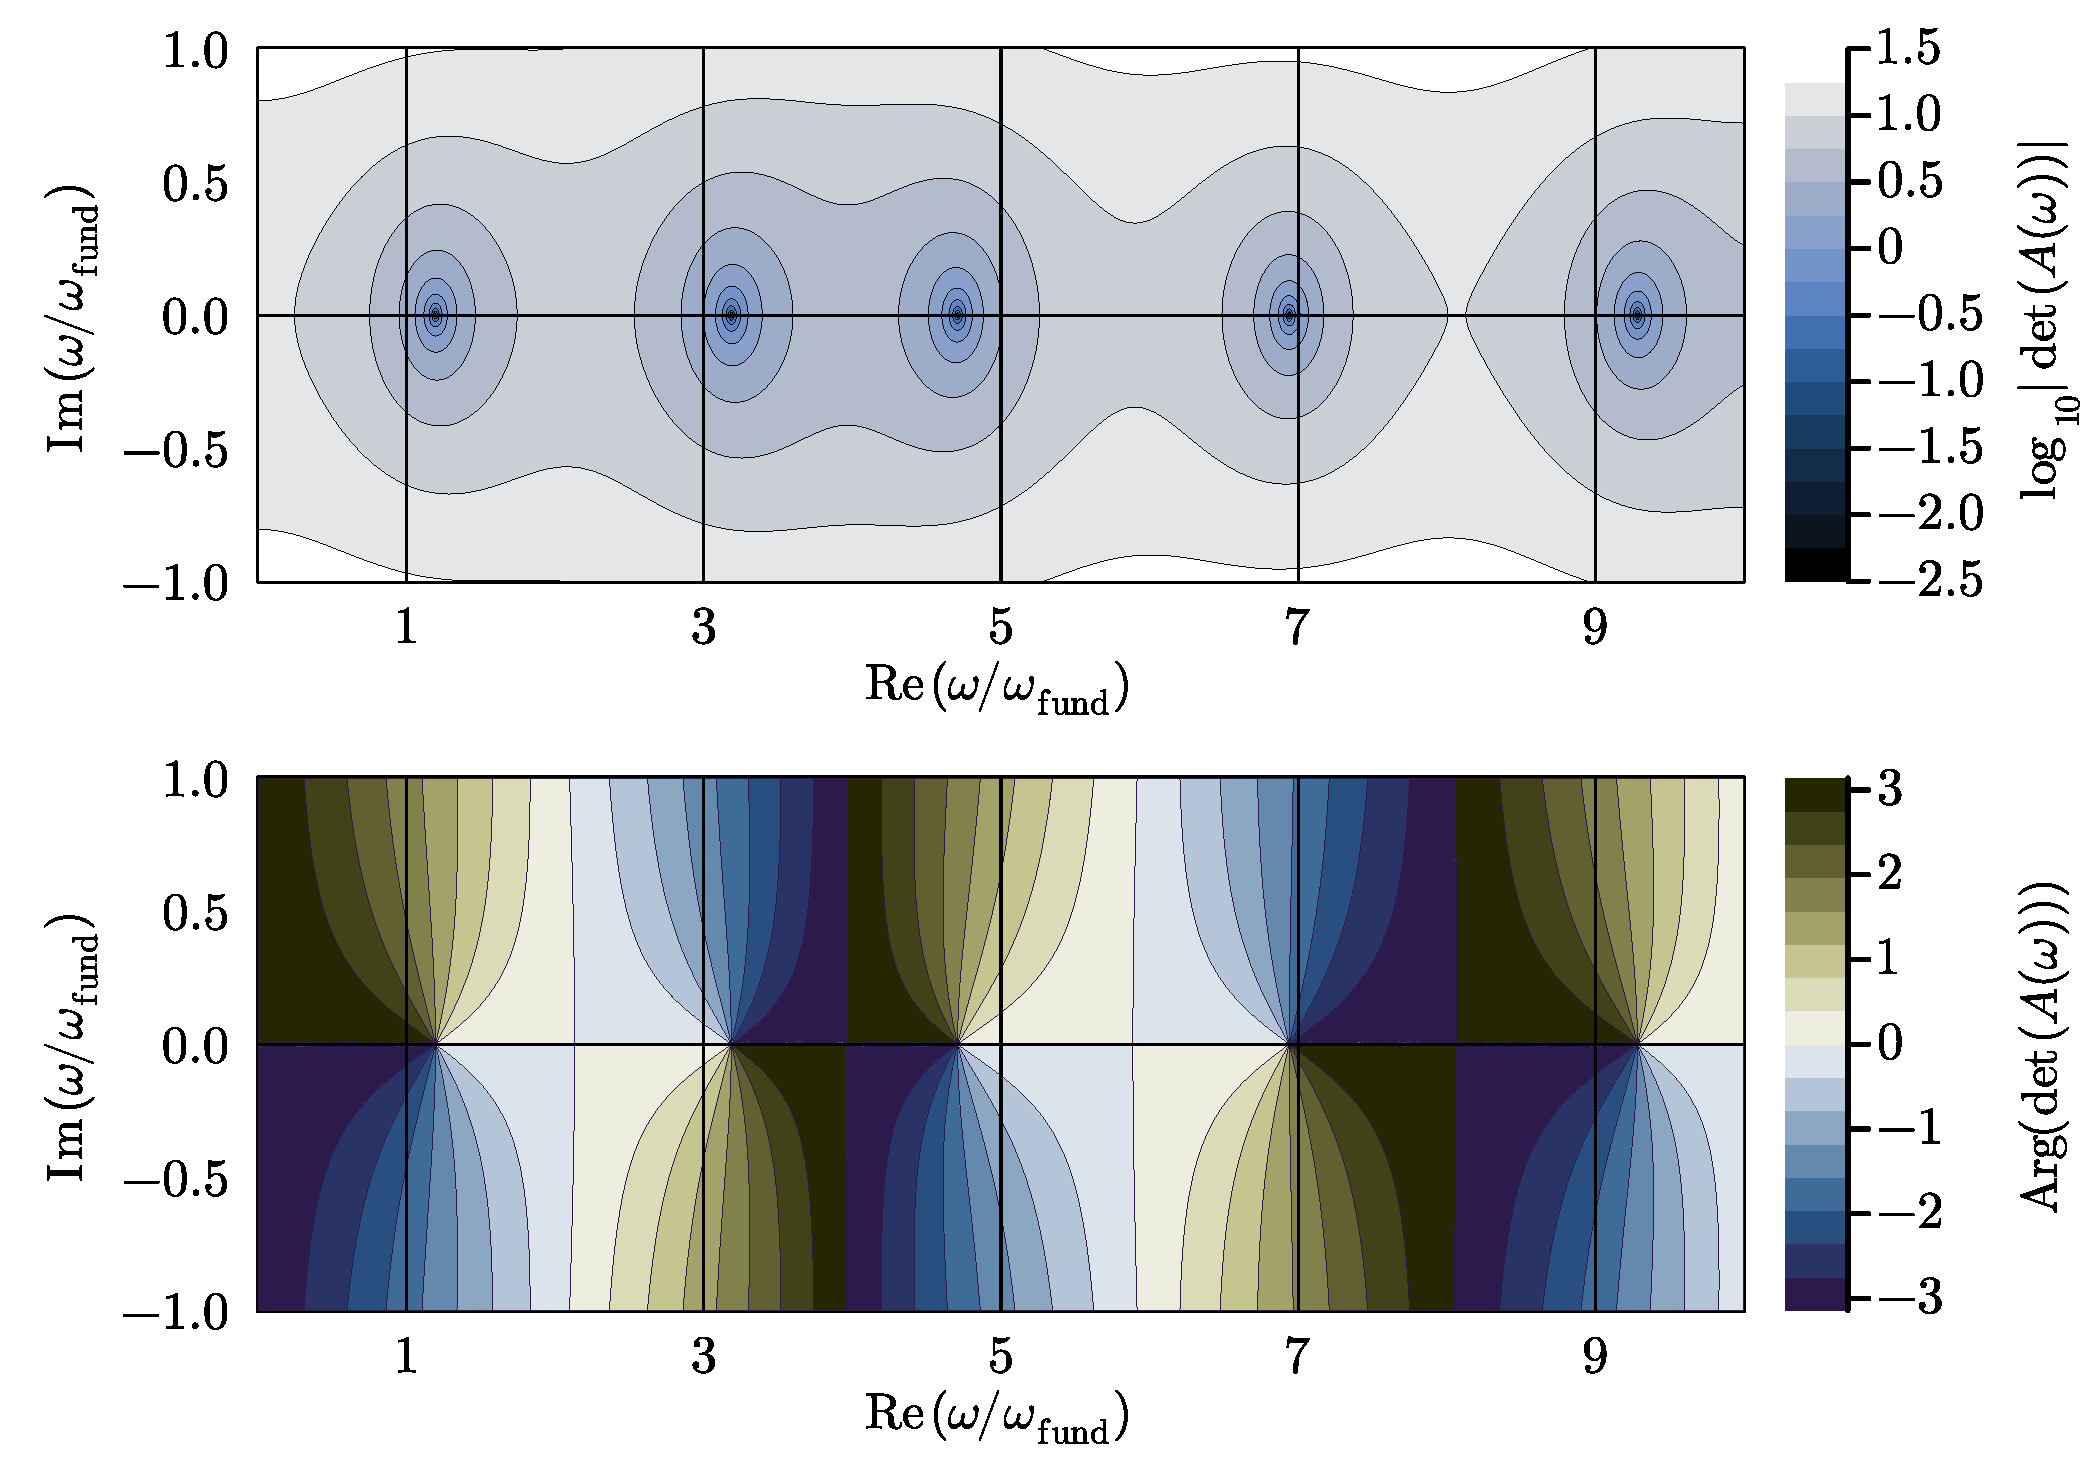
\includegraphics[scale=0.35]{assets/graphs/r=7_xf=05_complex_harmonics.pdf}
\caption{Values of $\det{A(ω)}$ for different values of $ω$ with $r = 7, x_f = 0.5$. Non-trivial solutions occur when $\abs{\det{A(ω)}} \ll 1$, which are seen in the darker regions of the plot.}
\label{fig:flame-harmonics-complex}
\end{subfigure}

\vspace*{0.5em}

\begin{subfigure}{0.99\textwidth}
\centering
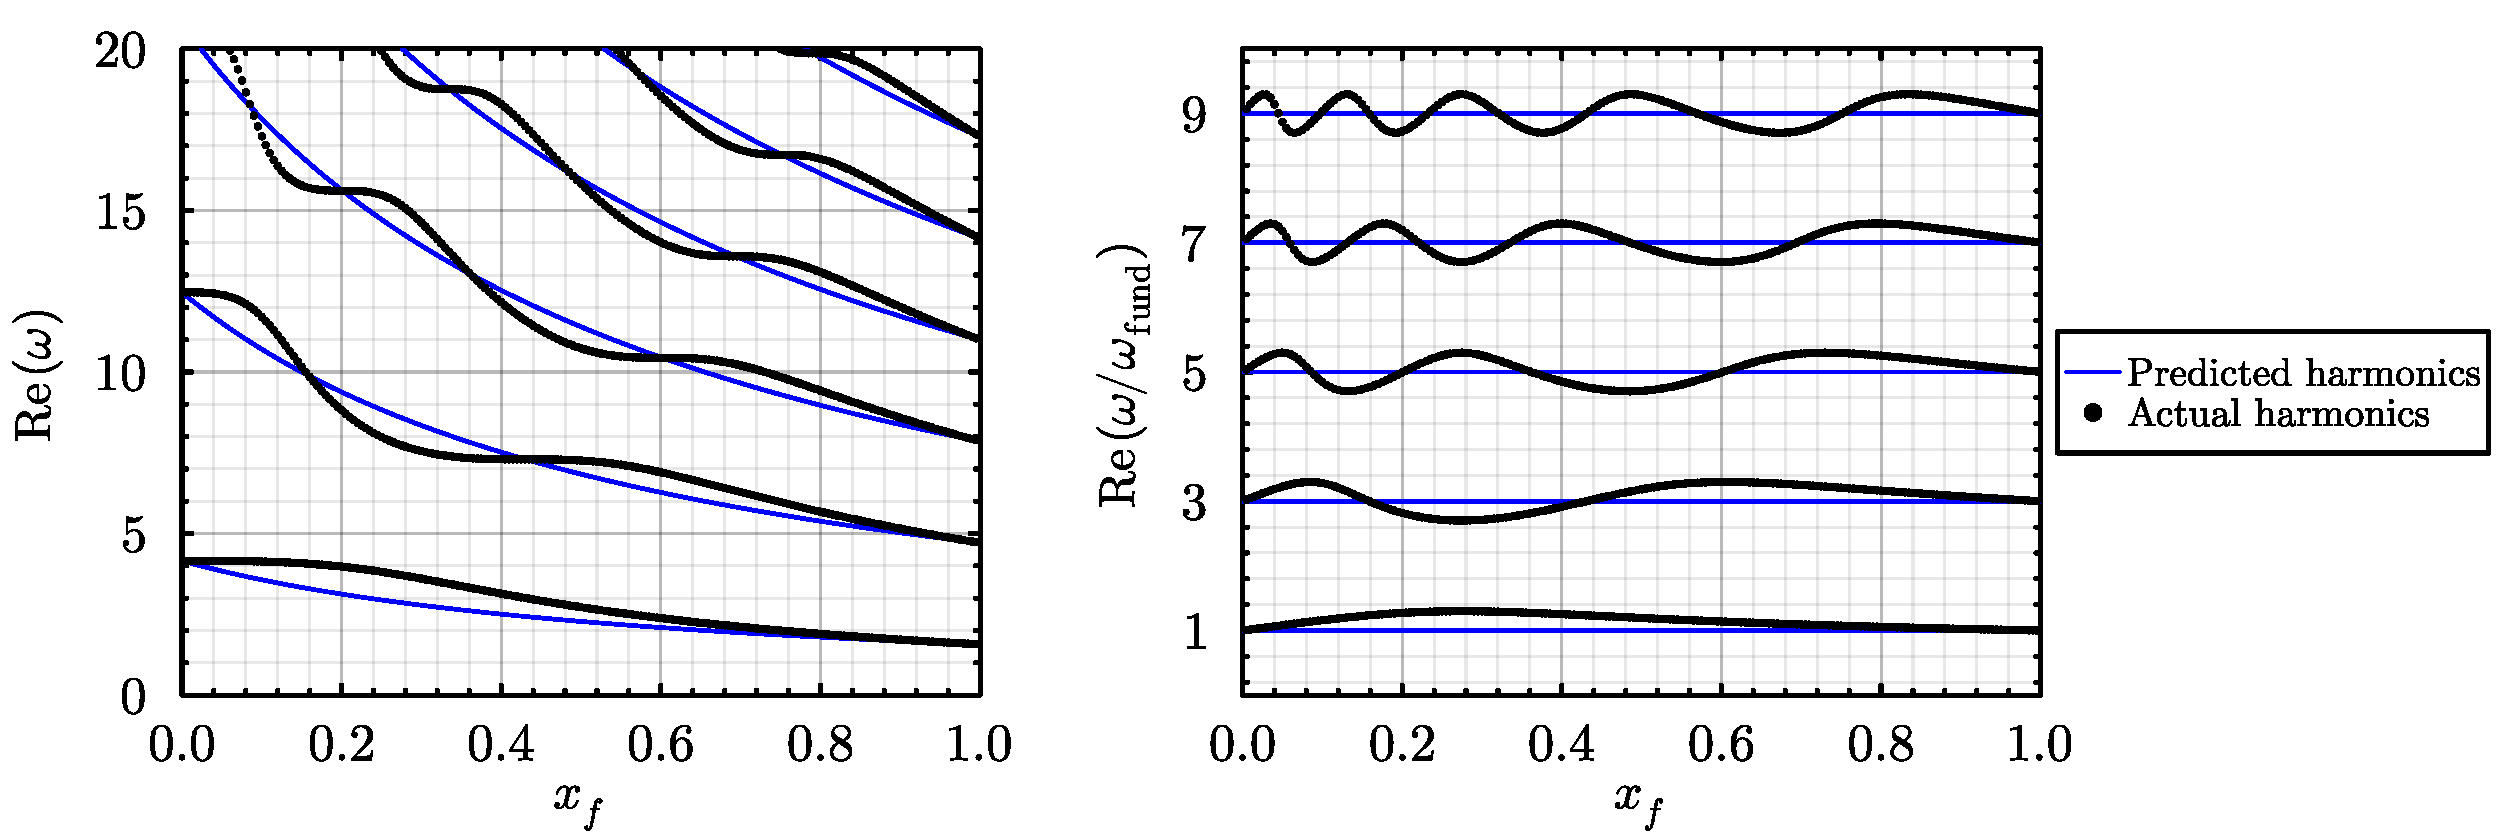
\includegraphics[scale=0.35]{assets/graphs/r=7_harmonics_both.pdf}
\caption{Predicted harmonics and true harmonics for $r = 7$ over a range of $x_f$ values.}
\label{fig:flame-harmonics}
\end{subfigure}
\caption{}
\label{fig:harmonics}
\end{figure}

For a flame where $x_f = 0.5$ and $r = 7$, we found that $ω_1 \approx 1.193 \, ω_{\rm{fund}}$ for the first harmonic and $ω_2 \approx 3.185 \, ω_{\rm{fund}}$. To transform these to dimensional variables, we must simply find the dimensional $\hat{ω}_{\rm{fund}}$. In a $\hat{l}_{\rm{tube}} = 1$ m long closed-open tube with $\hat{c}_{\rm{U}} \approx 348.15$ m s$^{-1}$, we get:
\begin{gather}
\hat{t}_{\rm{fund}} = \frac{\hat{l}_{\rm{tube}}}{\hat{c}_{\rm{U}}} \left( 4x_f  + \frac{4(1 - x_f)}{\sqrt{r}} \right)
\approx 7.92~\rm{ms}
\quad \text{so} \\
\hat{ω}_{\rm{fund}} = \frac{2π}{\hat{t}_{\rm{fund}}}
\approx 793.7~\rm{rad}~\rm{Hz}
\quad \text{and} \quad
\hat{f}_{\rm{fund}} = \frac{1}{\hat{t}_{\rm{fund}}}
\approx 126.3~\rm{Hz}
\end{gather}
where $\hat{f}$ if frequency and $\hat{ω}$ is angular frequency. The harmonics thus have dimensional frequency $\hat{f}_1 \approx 1.193 \, \hat{f}_{\rm{fund}} = 150.7$ Hz and $\hat{f}_2 \approx 3.185 \, \hat{f}_{\rm{fund}} = 402.4$ Hz.

Note that this analysis only accounts for the modes of a stationary density jump. If the flame were moving instead (as is the case for many thermoacoustically unstable flames in experimentation \cite{delfin2024ThermoacousticParametricInstability,delfin2024VideoTransientParametric, martinez-ruiz2018VideoPremixedflameOscillations}), the acoustic modes in the tube change with the moving flame. Hence the acoustics in the tube will be much more complex in this case in a way which is not predicted by this model. More complex control diagrams may be required to model the moving system as well as the coupled interaction of the flame with the acoustics, which is not explored here.

%%%% PLOT OF 1/4 and 3/4 EIGENMODE!!!!




\subsection{Simulation Results and Analysis}

We now investigate a thermoacoustically unstable flame in a 1 m long closed-open tube using ADCBC inflow and outflow. The DNS region is a similar rectangular region with symmetric top and bottom boundaries to before which is instead 2 cm by 2 mm, resolving the full flame and hydrodynamically active region. The reactant enters the domain with properties $u_{\rm{in}, 0} = 0.2$ m s$^{-1}$ (a counterflow flame), $T_0 = 298$ K and $p_0 = 1$ bar, as before. The upstream reactants $α = R$ and downstream products $α = P$ have the same properties as the gas from the previous inert test cases, except we specify a change in enthalpy of formation $Δ h_{f, R}^\plimsoll - Δ h_{f, P}^\plimsoll$ between the two such that the heat release parameter $q \equiv T_2 / T_1 - 1 = 6$. Species diffusion is modelled by a constant Lewis number approximation where $\Le = 1$ for both species. We use a single step reaction $\rm{R} \to \rm{P}$ with Zel'dovich number $\Ze = 5$ and Arrhenius reaction term $K_f = A\exp(-E_a / R_0 T)$. The constants $A$ and $E_a$ are chosen such that the laminar flame speed is $S_L = 0.2$ m s$^{-1}$. The resulting laminar flame thickness is $l_L \approx 0.216$ mm. It may seem like a large jump to go from a simulation of inert acoustics to fully reacting flame-acoustic interactions, but the sunset code is designed with flame simulations in mind, so the simulations are `easy' to perform having already implemented ADCBCs.

To discretise the interior of the domain, $k = 6$ is used for non-hyperviscosity differential operators, and $k_{\rm{HV}} = 8$ is used for $Δ^3$ hyperviscosity operators. The orders of these approximations drops for the boundary discretisation (see \cite{king2022HighOrderSimulationsIsothermal} for more details). Discretisation error should be dominated by the $\cl{O}(h^{k_{\rm{HV}} - 6 + 1}) = \cl{O}(h^{3})$ error in hyperviscosity operators. Even though LABFM enables variable discretisation resolutions, we use a constant resolution in the DNS domain as we don't know a priori where the flame will end up. A discretisation length scale of $s = 18$ {\textmu}m is used, resulting in a computational domain consisting of $\sim$50,000 discretisation points decomposed onto 52 processors of a single AMD Genoa compute node. As far as wallclock runtime is concerned, simulations are bottlenecked by the gradient and Laplacian calculations, where $\sim$50 nodes are in each stencil for interior nodes. As mentioned at the beginning of the chapter, a simple improvement to runtime is to simply use a high-order centred finite difference scheme on a rectangular lattice with similar hyperviscosity filtering for stability. This will, however, not be an option when we move on to simulating complex DNS geometries (although this is not explored in this report) where unstructured meshing is traditionally a requirement.

The flame is initialised in its two-dimensional curved steady state by first running a simulation in the same computational domain with the same flame and fluid properties with non-reflecting NSCBC inflow and outflow boundaries. The flame is placed toward the right of the DNS domain such that the flame has more room to move leftward as it curves, increasing its flame speed $S_c$.

\begin{figure}[t]
\centering
\begin{subfigure}{0.99\textwidth}
\centering
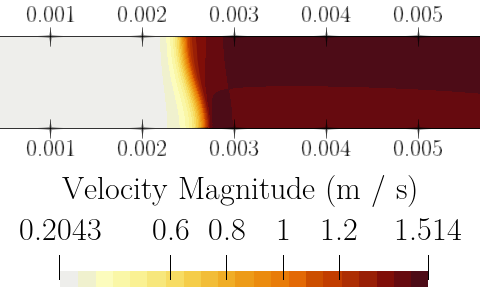
\includegraphics[scale=0.36]{assets/graphs/THERMOAC_mag-v.png}
\caption{Velocity magnitudes in the hydrodynamic zone surrounding the flame at the end of the simulation. Notice that although we have $\overline{u}_{\rm{IN}} = 0.2$ m s$^{-1}$ and $\overline{u}_{\rm{OUT}} = r \, \overline{u}_{\rm{IN}}$ (where $r = 7$ for this flame), the values shown are higher due to a positive contribution from the acoustics $u_a > 0$ in the DNS region.}
\label{fig:mag-v}
\end{subfigure}

\vspace*{0.5em}

\begin{subfigure}{0.99\textwidth}
\centering
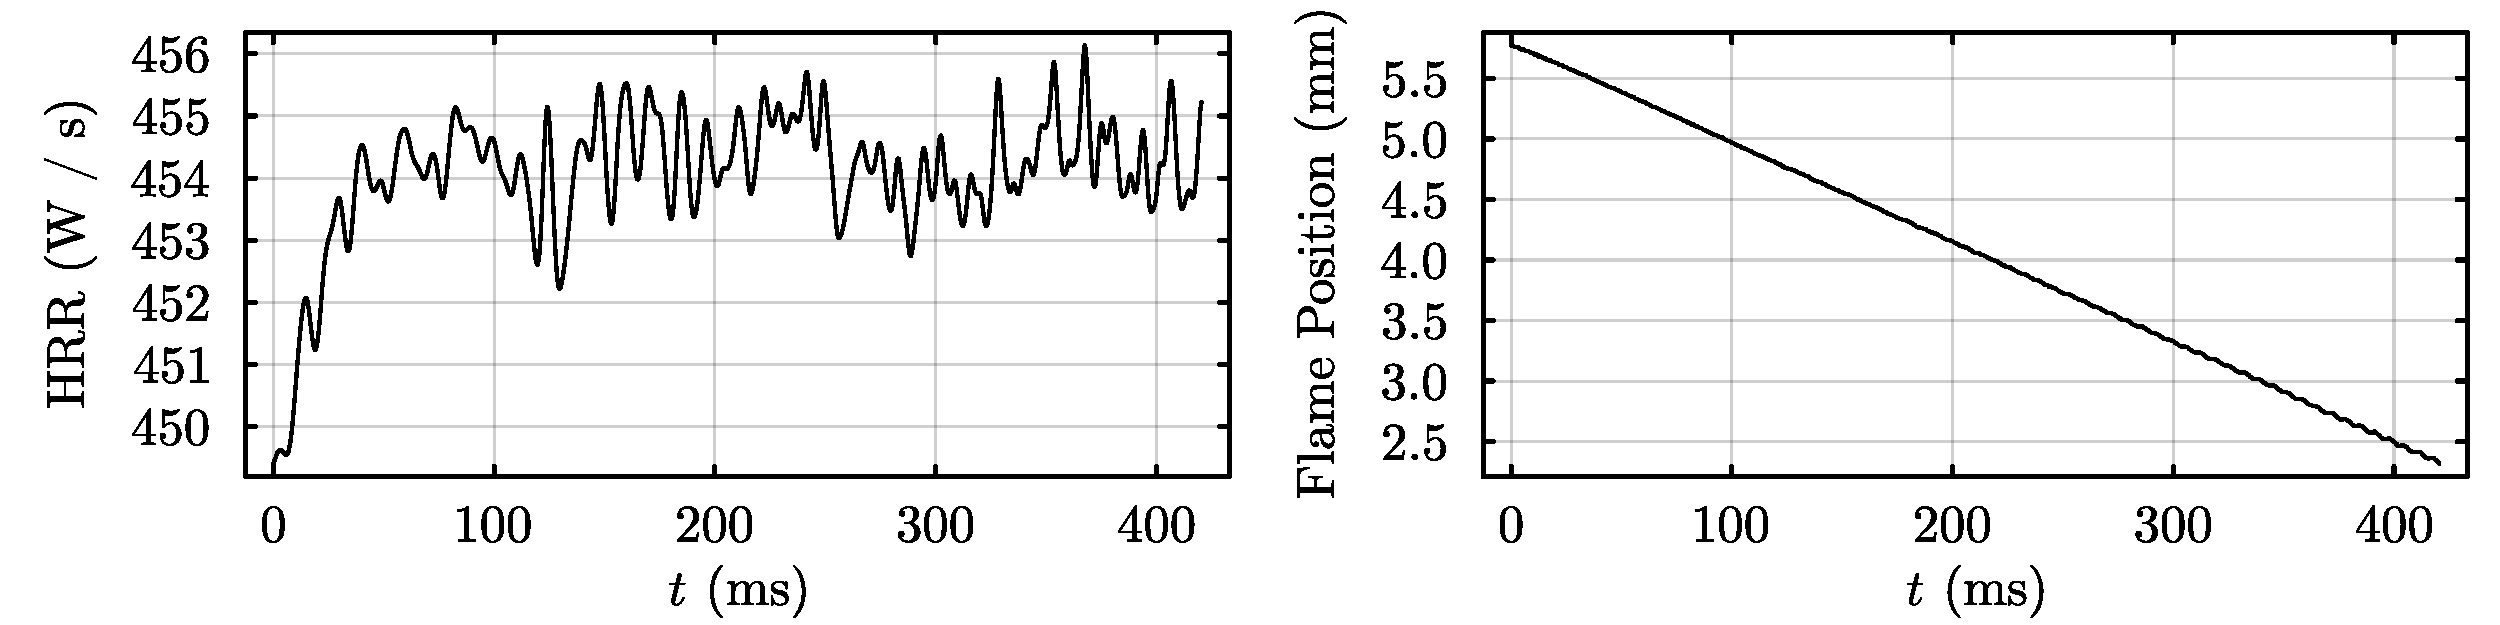
\includegraphics[scale=0.35]{assets/graphs/2mmx1m_still_hrr-flame.pdf}
\caption{Time series' of (left) integrated Heat Release Rate (HRR) in the DNS region and (right) leftmost flame position.}
\label{fig:hrr-flame}
\end{subfigure}
\caption{}
\label{fig:flame}
\end{figure}

Unfortunately, as of submitting this report, the thermoacoustic mode in these simulations has not fully developed, so results shown are only preliminary. However, they should exemplify the ability of ADCBCs to accurately reconstruct the expected acoustic behaviour. Because of this early stage, the final flame structure shown in \fig{fig:mag-v} is the result primarily of the Darrieus-Landau (DL) instability and closely matches that expected of two-dimensional simulations \cite{creta2011StrainRateEffects}. In the right of \fig{fig:hrr-flame}, the acoustic displacement of the flame results in very small but noticeable `wobbling'.\footnote{You may have to zoom in!} The heat release shown in the left graph appears to be much more aperiodic in nature. This is most likely the result of the complex interaction of the flame to the surrounding acoustic field on top of the DL mode.


\begin{figure}[t]
\begin{subfigure}{0.99\textwidth}
\centering
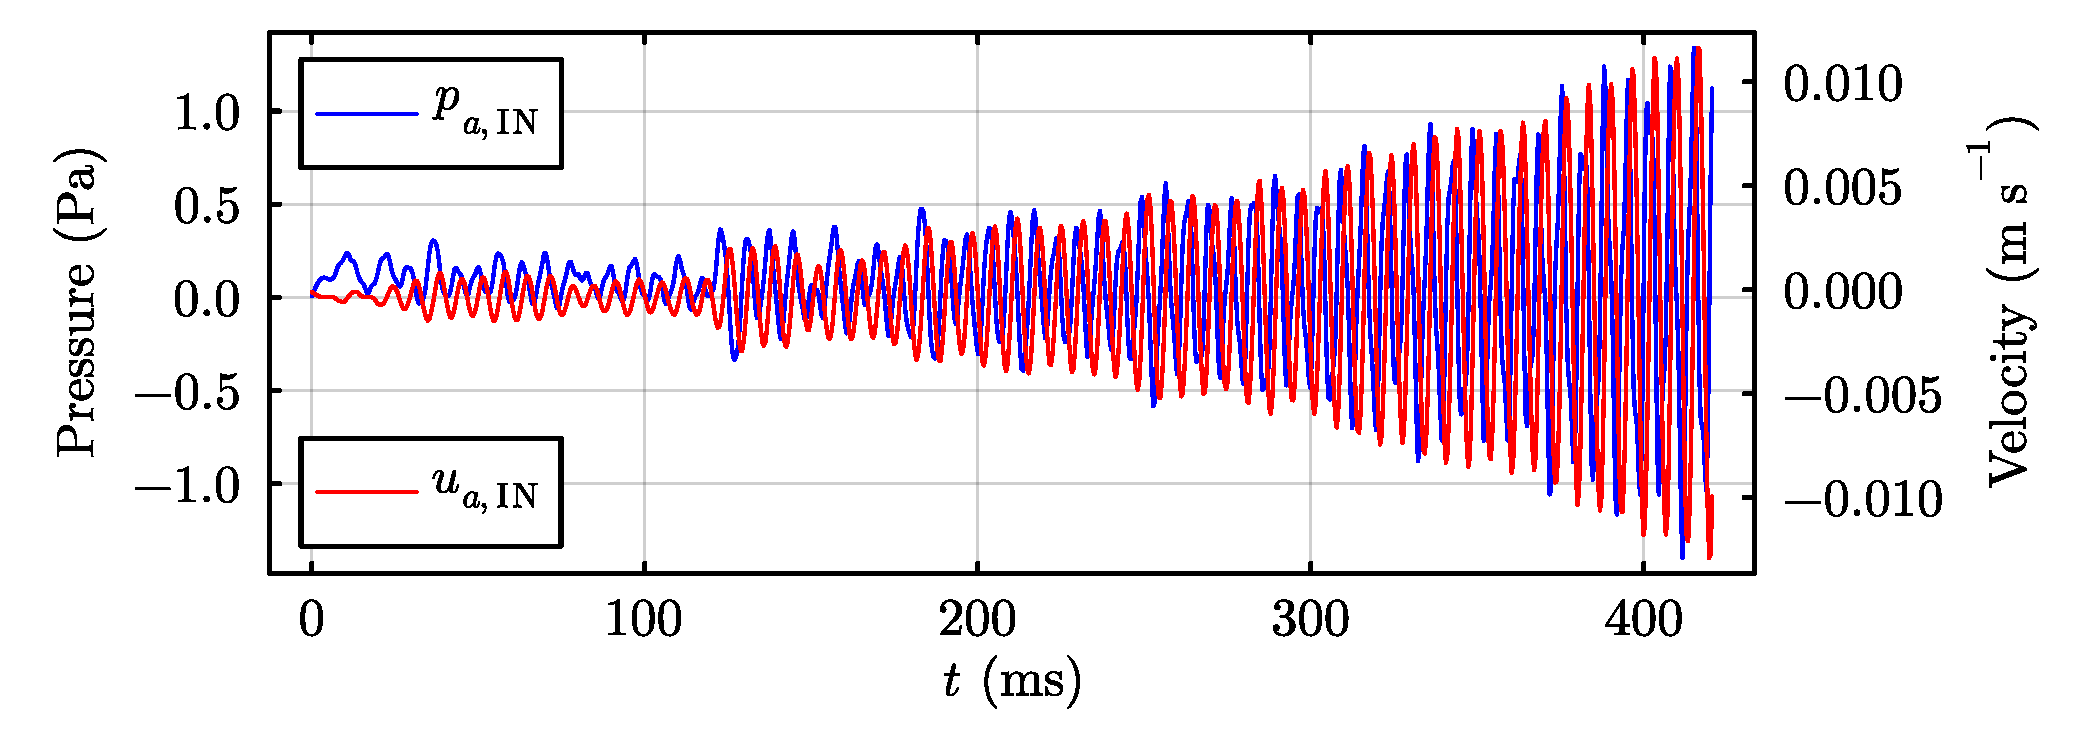
\includegraphics[scale=0.35]{assets/graphs/2mmx1m_still_pu.pdf}
\caption{Time series of acoustic pressure and velocity values at the ADCBC inflow.}
\label{fig:2mmx1m_still_pu}
\end{subfigure}

\vspace*{0.5em}

\begin{subfigure}{0.99\textwidth}
\centering
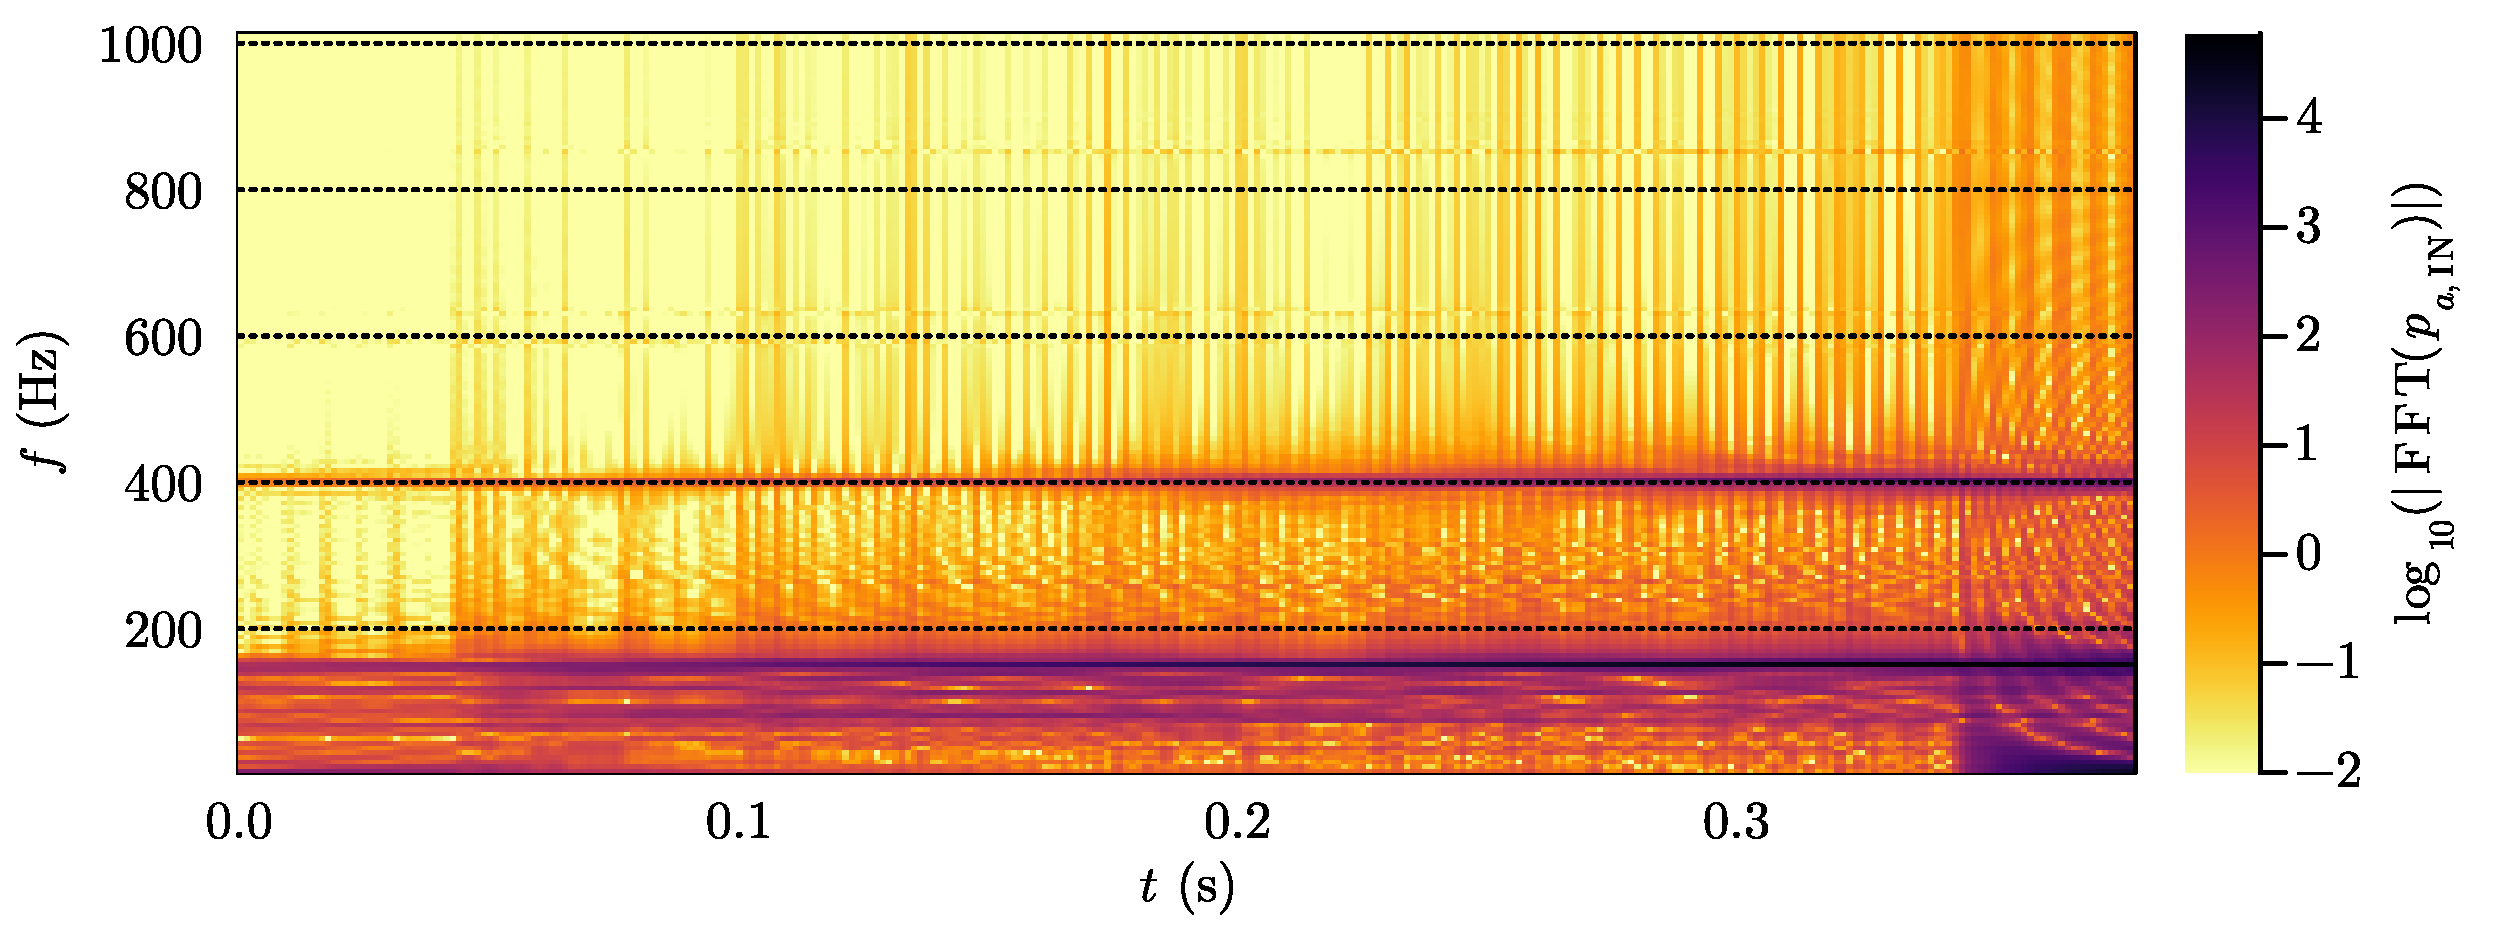
\includegraphics[scale=0.35]{assets/graphs/2mmx1m_still_spec2.pdf}
\caption{Spectrogram of acoustic pressure values at the ADCBC inflow. The final $\sim$0.03 s has spuriously higher mode amplitudes due to zero padding used at the end of the time series.}
\label{fig:spectrogram}
\end{subfigure}
\caption{}
\label{fig:in-ac}
\end{figure}

\begin{figure}[t]
\centering
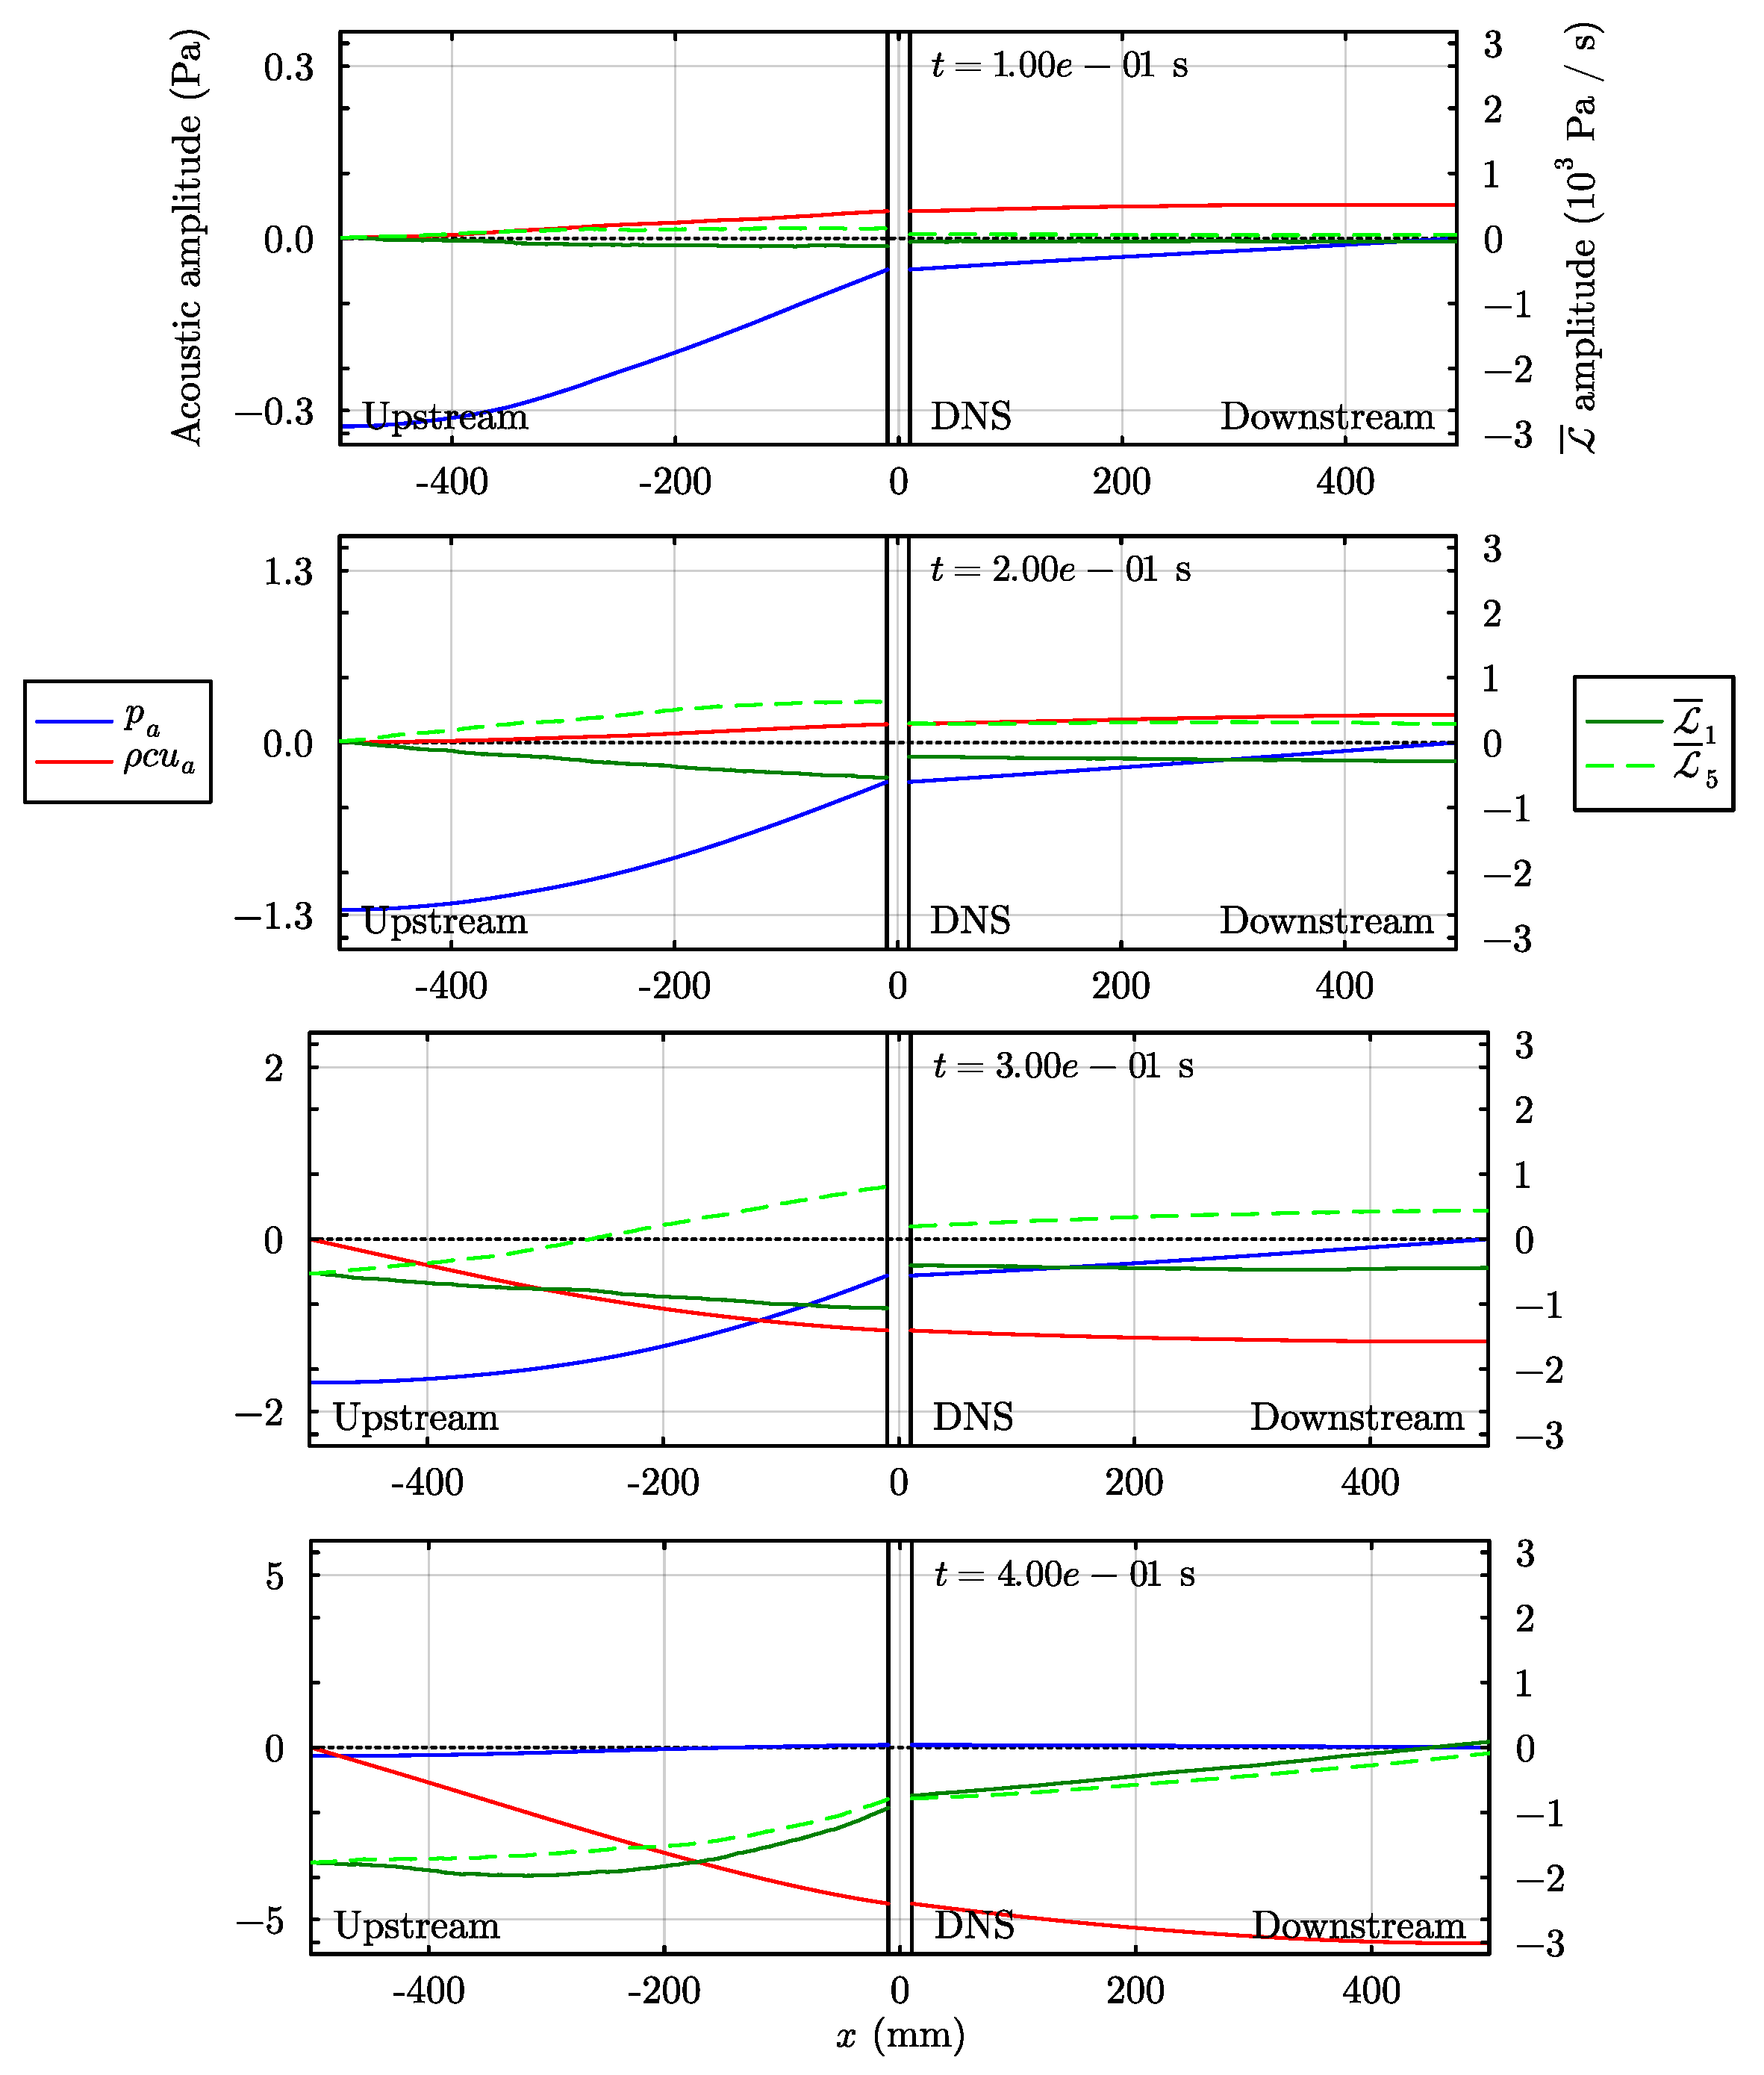
\includegraphics[scale=0.35]{assets/graphs/2mmx1m_still_ac.pdf}
\caption{Reconstruction of the acoustic fields for this flame simulation at times $t = 0.1, 0.2, 0.3$ and 0.4 s. The reconstructed fields $p_a$ and $u_a$ are translated vertically here such that $p_a(x_{\rm{OUT}} + l_{\rm{D}}) = 0$, $u_a(x_{\rm{IN}} - l_{\rm{U}}) = 0$, $p_a(x_{\rm{IN}}) = p_a(x_{\rm{OUT}})$ and $u_a(x_{\rm{IN}}) = u_a(x_{\rm{OUT}})$. These boundary conditions do not match those defined in the previous chapter, and are just used for simpler visualisation since the non-acoustic pressure and velocity are different on either side of the flame.}
\label{fig:thermoac-reconstruct}
\end{figure}

In \fig{fig:2mmx1m_still_pu} we show the acoustic pressure and velocity at the ADCBC inflow over the course of the simulation. We can clearly see the growth of the primary instability in the acoustic envelope. When this primary thermoacoustic mode is fully developed, we expect the flame to quickly flatten and for the acoustic amplitude to plateau as the instability reaches a limit cycle. To predict growth rate and onset of secondary instability, one could also calculate the Rayleigh index RI introduced in \chap{ch:lit-review}, although this analysis is not performed here. True growth rates can also be calculated by finding the envelope of the acoustic data shown in \fig{fig:2mmx1m_still_pu} since $\log(\rm{env}(t)) \propto -ω_i t$ where $-ω_i$ is the growth rate and the function $\rm{env}(t)$ defines the acoustic envelope for these inflow acoustics. Increasing the growth rate of these modes in future simulations would allow us to reach and study the thermoacoustic instability faster. A spectrogram of this data is shown in \fig{fig:spectrogram}, where large spikes are seen across the whole simulation for $f_1 = \sim$150 Hz and $f_2 = \sim$400 Hz. These are very close to the frequencies predicted by the acoustic analysis in the previous section! We note, however, that we expect the interaction of the acoustics with the flame to modulate the resonating frequency \cite{silva2023IntrinsicThermoacousticInstabilities}. This remains unexplained as acoustic-flame coupling is not explored in the acoustic model. The dominance of the perturbed 1/4 mode in the acoustic fields is shown in \fig{fig:thermoac-reconstruct}, where the 1/4 mode can be seen clearly in each snapshot of the acoustic field. Note that although the 3/4 mode is also present, its amplitude is at least one order of magnitude throughout the simulation. This makes it difficult to observe in the full acoustic reconstruction.

